\section{Experimental Results}
    In this section, we first present the overall success rate for cracking
    the 120 patterns collected from our participants plus the top 60 most complex patterns
    on a $3\times3$ pattern grid.
    Our results show that the attack can successfully crack over 95\% of the
    patterns using no more than five attempts. We then analyze how the
     success rate is affected by various filming conditions: the filming distance and angle,
    the camera shake effect, lighting, the screen size of the mobile device, and the filming cameras. Next, we evaluate our approach on alternative pattern grids and demonstrate that direct observations have lower success rates compared to our attack.
    We conduct a limited study to understand how our attack performs when the video only captures the user's fingertip.
     Finally, we demonstrate that our video-based attack can also be used to crack PIN-based passwords.

\begin{figure}[!t]
    \centering
    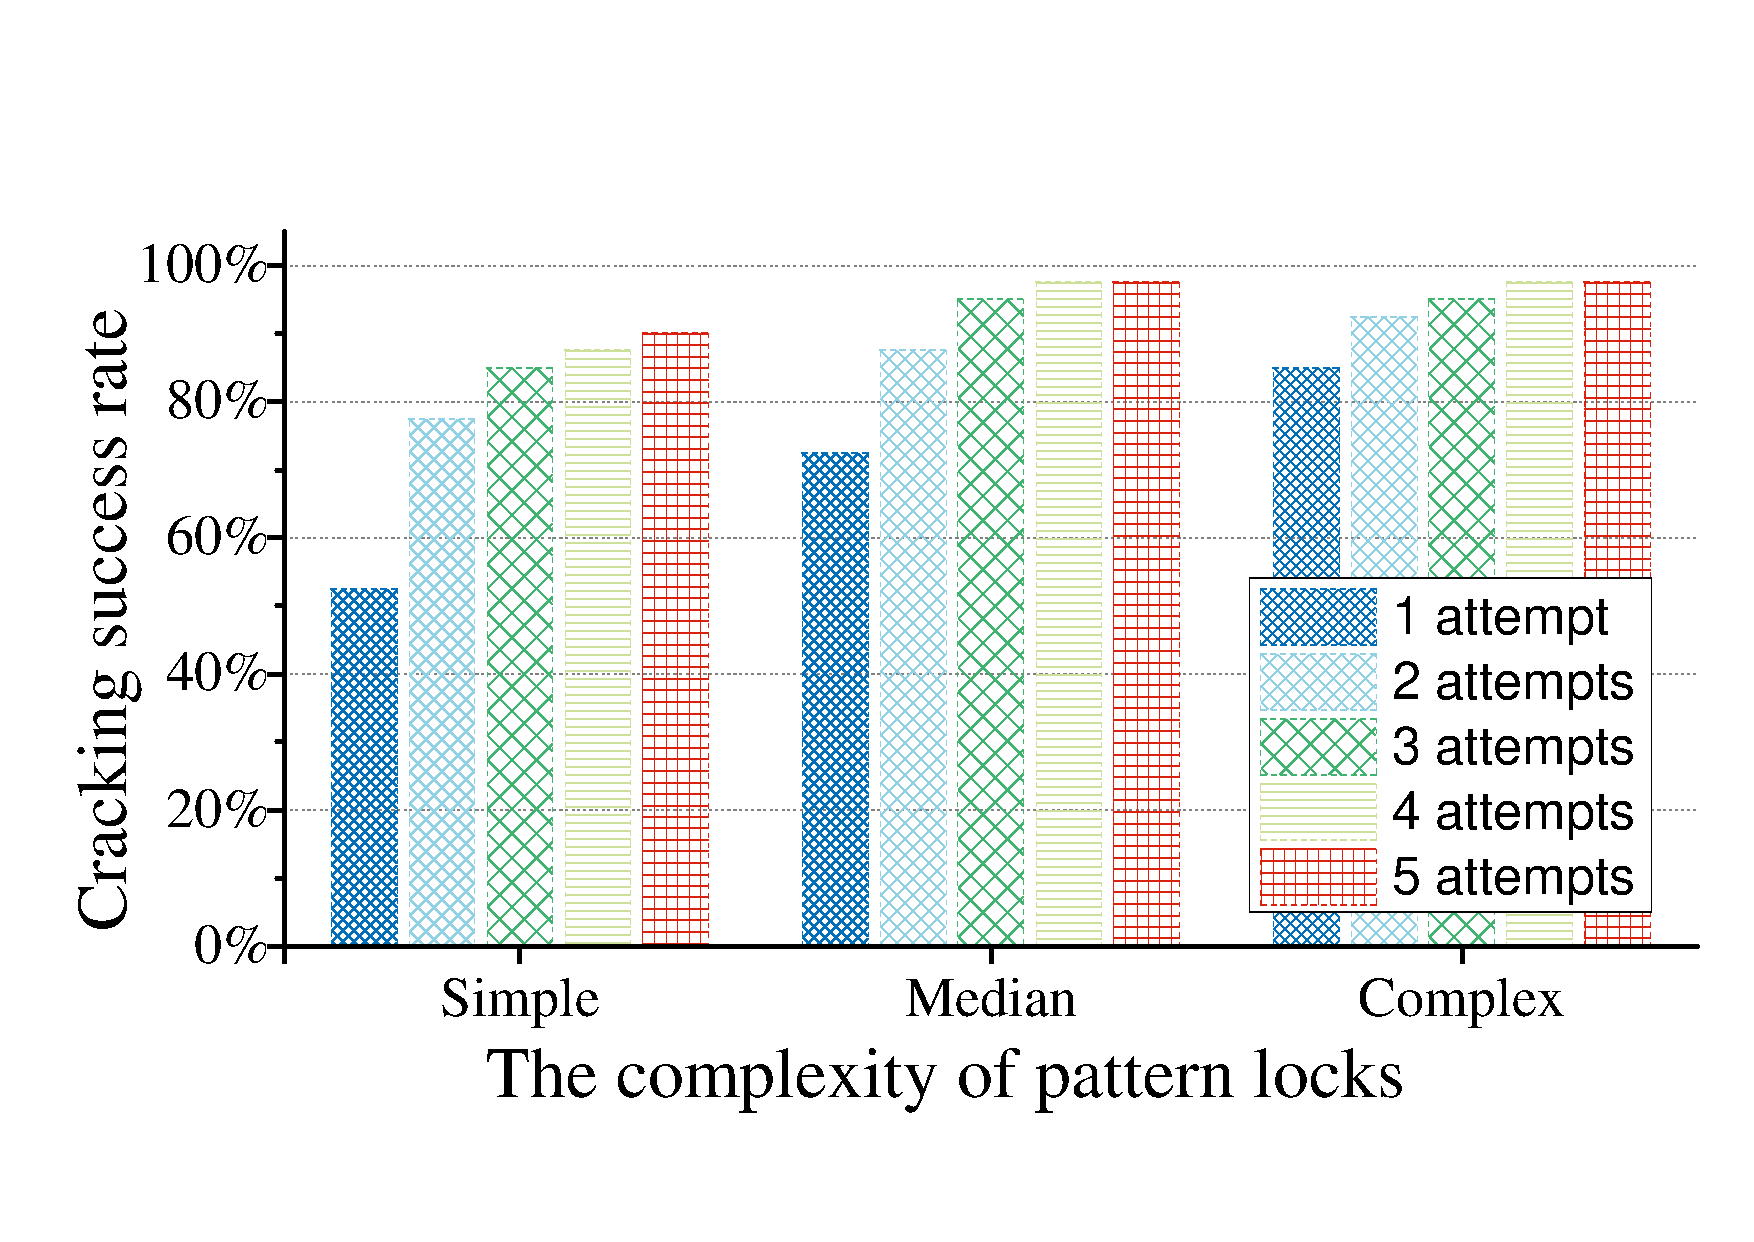
\includegraphics[width=0.5\textwidth]{fig/10.pdf}
    \caption{For each pattern category, the figure shows the success rate using no more than 1, 2, 3, 4 and 5 attempts.}
    \label{fig:fig10}
\end{figure}

    \subsection{Overall Success Rate \label{sec:overall_rate}}

    \noindent \textbf{Result 1:}  \emph{We can successfully crack over 95\% of the patterns in five attempts and complex patterns are less secure compared to simple patterns under our attack.}


        In this experiment, videos were recorded from a distance of 2 meters away
        from the target device. This mimics a scenario where the adversary sits
        at the next table to the user in a public space (e.g. a restaurant).
        The smartphones used for filming in this experiment were hand-held.

        \subsubsection{Evaluation using collected user patterns}
        Figure~\ref{fig:fig10}
        shows the success rate for cracking different types of patterns within 1, 2, 3, 4 and 5 attempts.
        We used the 120 patterns that have been collected through our user studies in this experiment.
        For all the patterns used in this evaluation,
        our approach does not generate more than  five candidate patterns.
        For complex patterns, we are able to crack all except one (with a 97.5\% success rate) \emph{in the first attempt}.
        For simple and median patterns, the success rate increases with more tries.
        In one attempt, we are able to
        successfully crack 60\% and 87.5\% of the simple and median patterns respectively. With two attempts, the success rate increases to 87.5\%,
        and 95\% for simple and median patterns
        respectively. Using five attempts, we are able to
        crack all simple patterns and all but one median patterns.
       The reason that we failed on one median and one complex patterns is because of some blur motions of the video footage (probably
       caused by the video compressing algorithm), which leads
       to many tracking failures. But we are able to crack the same
       pattern using a video filmed by a different device.
        It is important to note that the native Android system allows up to five failed tries before locking the device~\cite{egelman2014you}. This means, in practice, our approach is able to
        successfully crack most locking patterns.

\begin{figure}[!t]
    \centering
    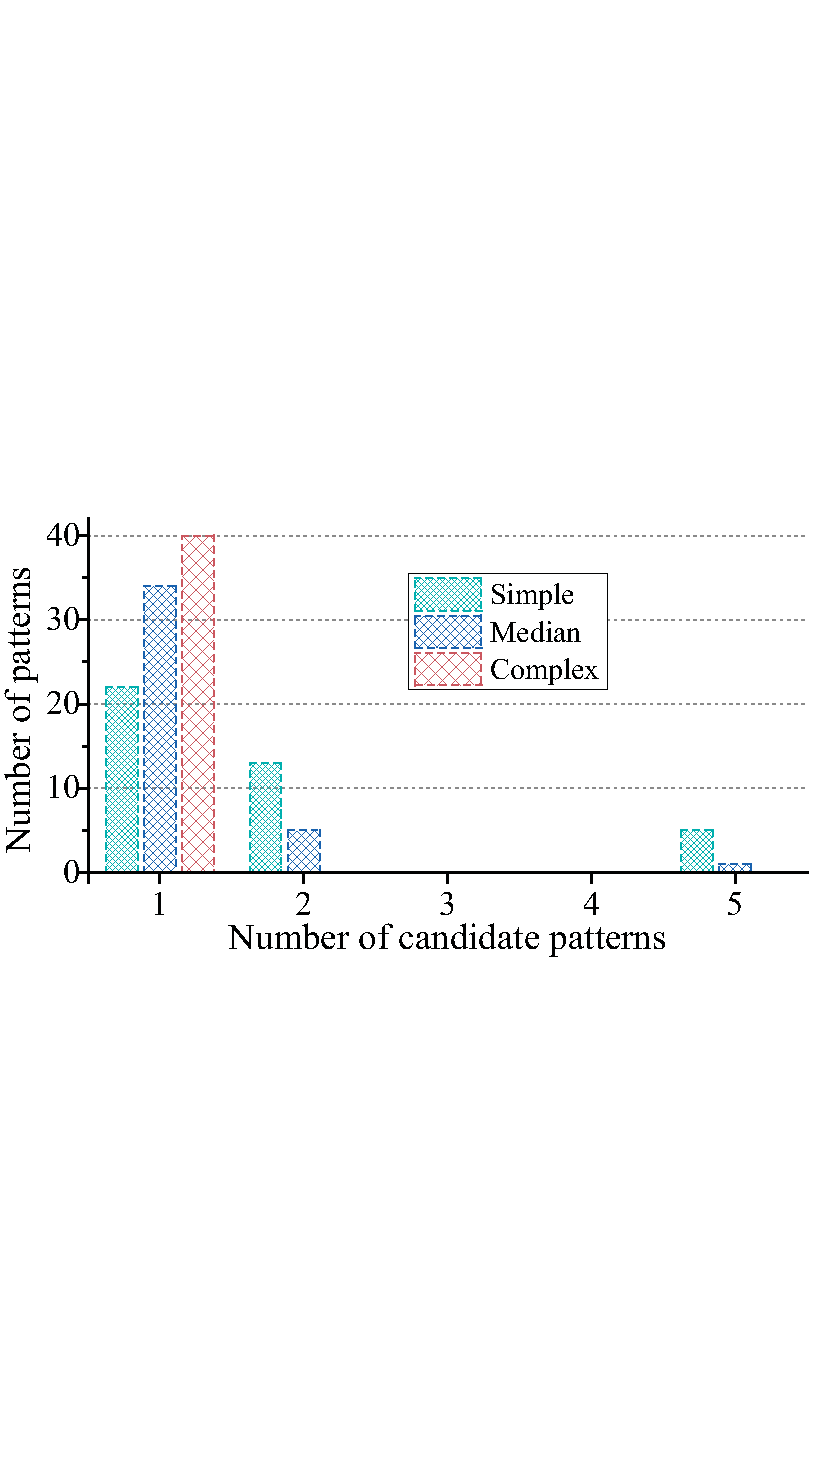
\includegraphics[width=0.5\textwidth]{fig/11.pdf}
    \caption{The distribution of candidate patterns for each category. No more than 5 candidate patterns were generated by our algorithm. }
    \label{fig:fig11}
\end{figure}

        Another interesting observation is that in contrast to many people's
        intuition, complex patterns do not provide stronger protection under our attack -- as can be seen by the fact that
        most of the complex patterns can be cracked in one attempt.
        This is because although complex patterns can better protect the user against direct observation techniques like shoulder surfing~\cite{shoulder}, their unique graphical structures
        help our algorithms to narrow the possible options down. This is
        confirmed by Figure~\ref{fig:fig11}. It shows that for most median and all complex patterns, our system produces one candidate pattern --
        the correct one for most of our test cases.




        \begin{figure}[!t]
            \centering
            \subfigure{
                \begin{minipage}[b]{0.12\textwidth}
                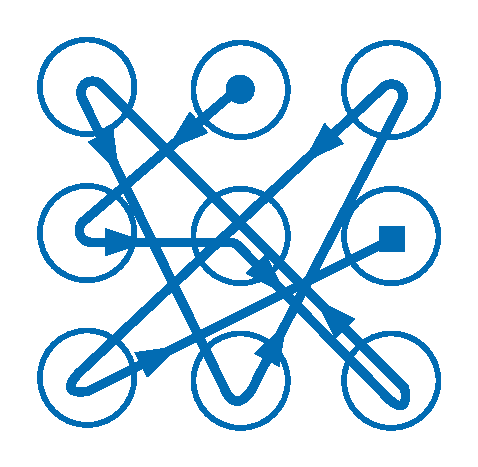
\includegraphics[width=\textwidth]{fig/complex3.pdf} \\
                \centering  complexity score: $43.8$
                \end{minipage}
            }
            \subfigure{
                \begin{minipage}[b]{0.12\textwidth}
                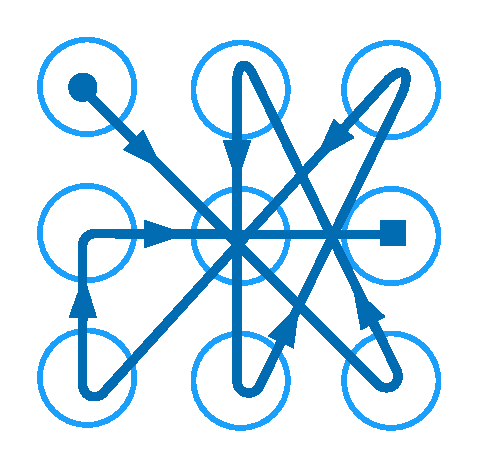
\includegraphics[width=\textwidth]{fig/complex2.pdf} \\
                \centering  complexity score: $44.7$
                \end{minipage}
            }
            \subfigure{
                \begin{minipage}[b]{0.12\textwidth}
                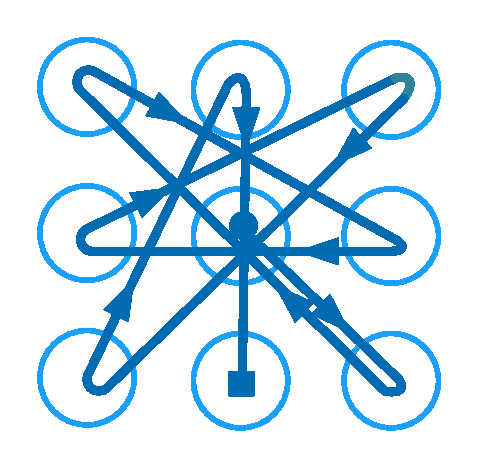
\includegraphics[width=\textwidth]{fig/complex1.pdf} \\
                \centering  complexity score: $46.8$
                \end{minipage}
            }
            \caption{Three most complex patterns on a $3\times 3$ grid based on Equation~\ref{equ:compscore}.}
            \label{fig:most complex patterns}
        \end{figure}

     \subsubsection{Evaluation on the most complex patterns}
       We also evaluated our approach using the top 60 most complex
        patterns (according to Equation~\ref {equ:compscore}) on a $3 \times 3$
        grid.
        To evaluate our approach on a wide range of patterns, we exclude patterns that are simply a rotation to an already chosen pattern.
         Figure~\ref{fig:most complex patterns} illustrates three
        highly complex patterns which have a complexity score between 43.8 and 46.8. The three
        patterns use all the nine dots of the grid and have a larger number of line segments, intersections and overlapping lines when compared to simpler patterns.
        Because of their complex graphical structures, remembering
        these patterns using direct observation techniques would be difficult.
        In this experiment, we can crack all the complex patterns in one attempt. This result reinforces our claim that complex
        patterns are less security under video-based attacks.


       \begin{figure}[!t]
            \centering
            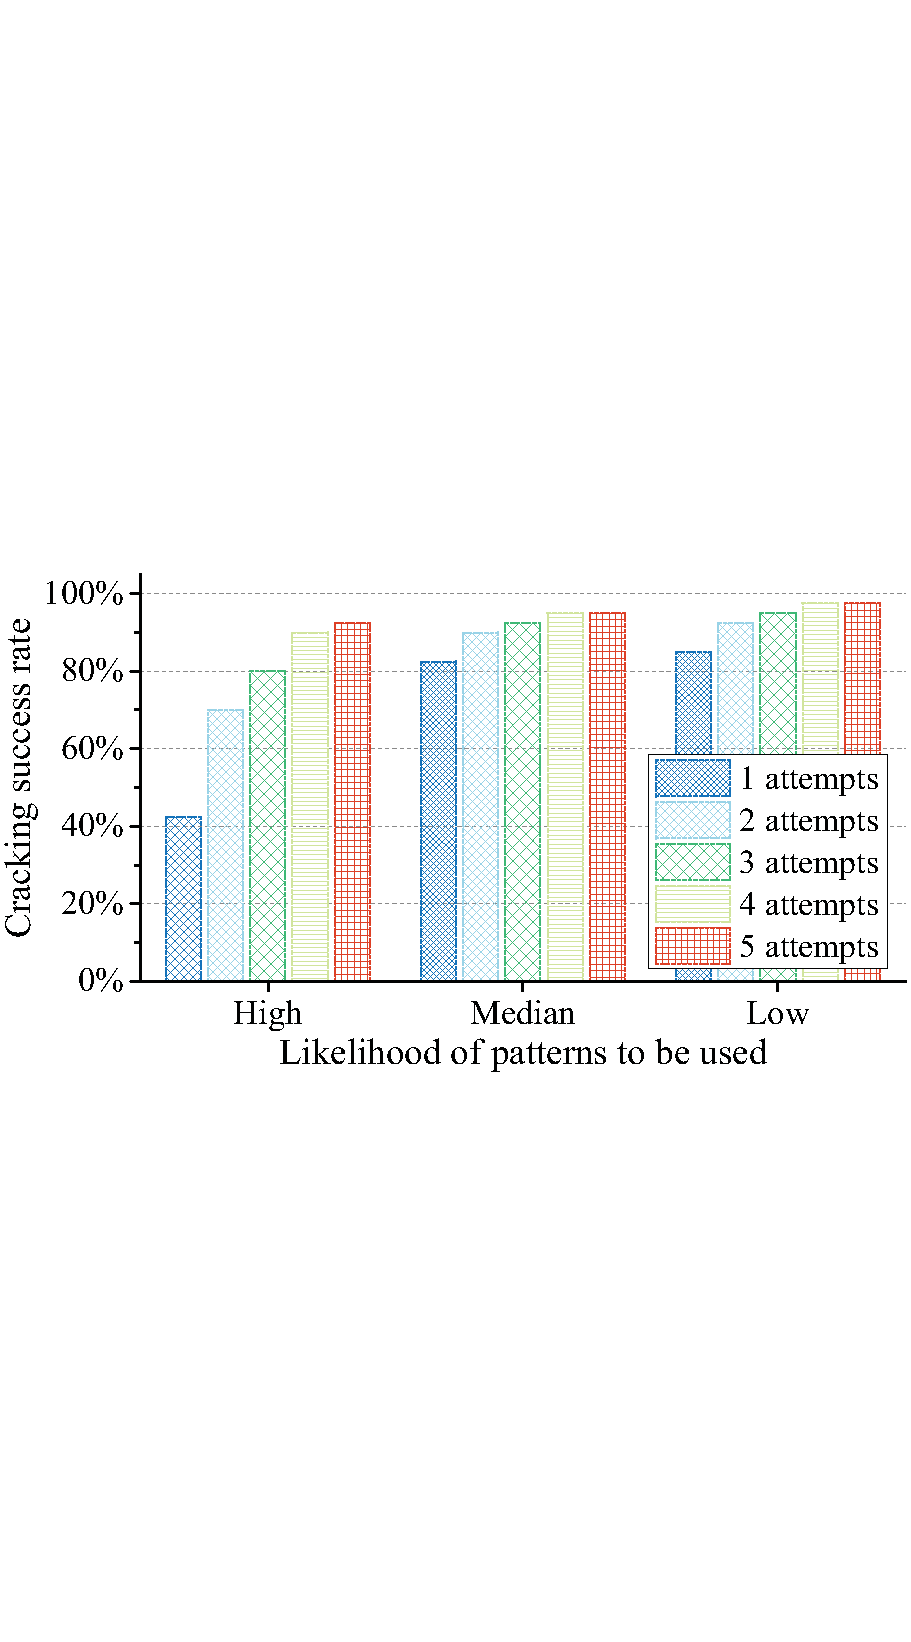
\includegraphics[width=0.5\textwidth]{fig/usibility_crackingNum.pdf}
            \caption{The attacking success rate when grouping patterns based on how likely a pattern will be used.
            The likelihood is calculated using Equation~\ref{equ:guessing_number}.}
            \label{fig:usage-crackingNum}
        \end{figure}

        \begin{table}[!t]
            \centering
            \caption{The repetition rate of two groups of patterns}
            \vspace{-0.2mm}
            \label{tab:repetition_rate}
            \scriptsize
            \begin{tabular}{cccc}
                \toprule
                \textbf{Group}& simple v.s. high & median v.s. median & complex v.s. low \\
                \midrule
                \textbf{reception rate}  & 72.5\% & 67.5\% & 80\% \\
                \bottomrule
            \end{tabular}
        \end{table}

         \begin{figure*}[!ht]
            \centering
            \subfigure{
                \begin{minipage}[b]{0.23\textwidth}
                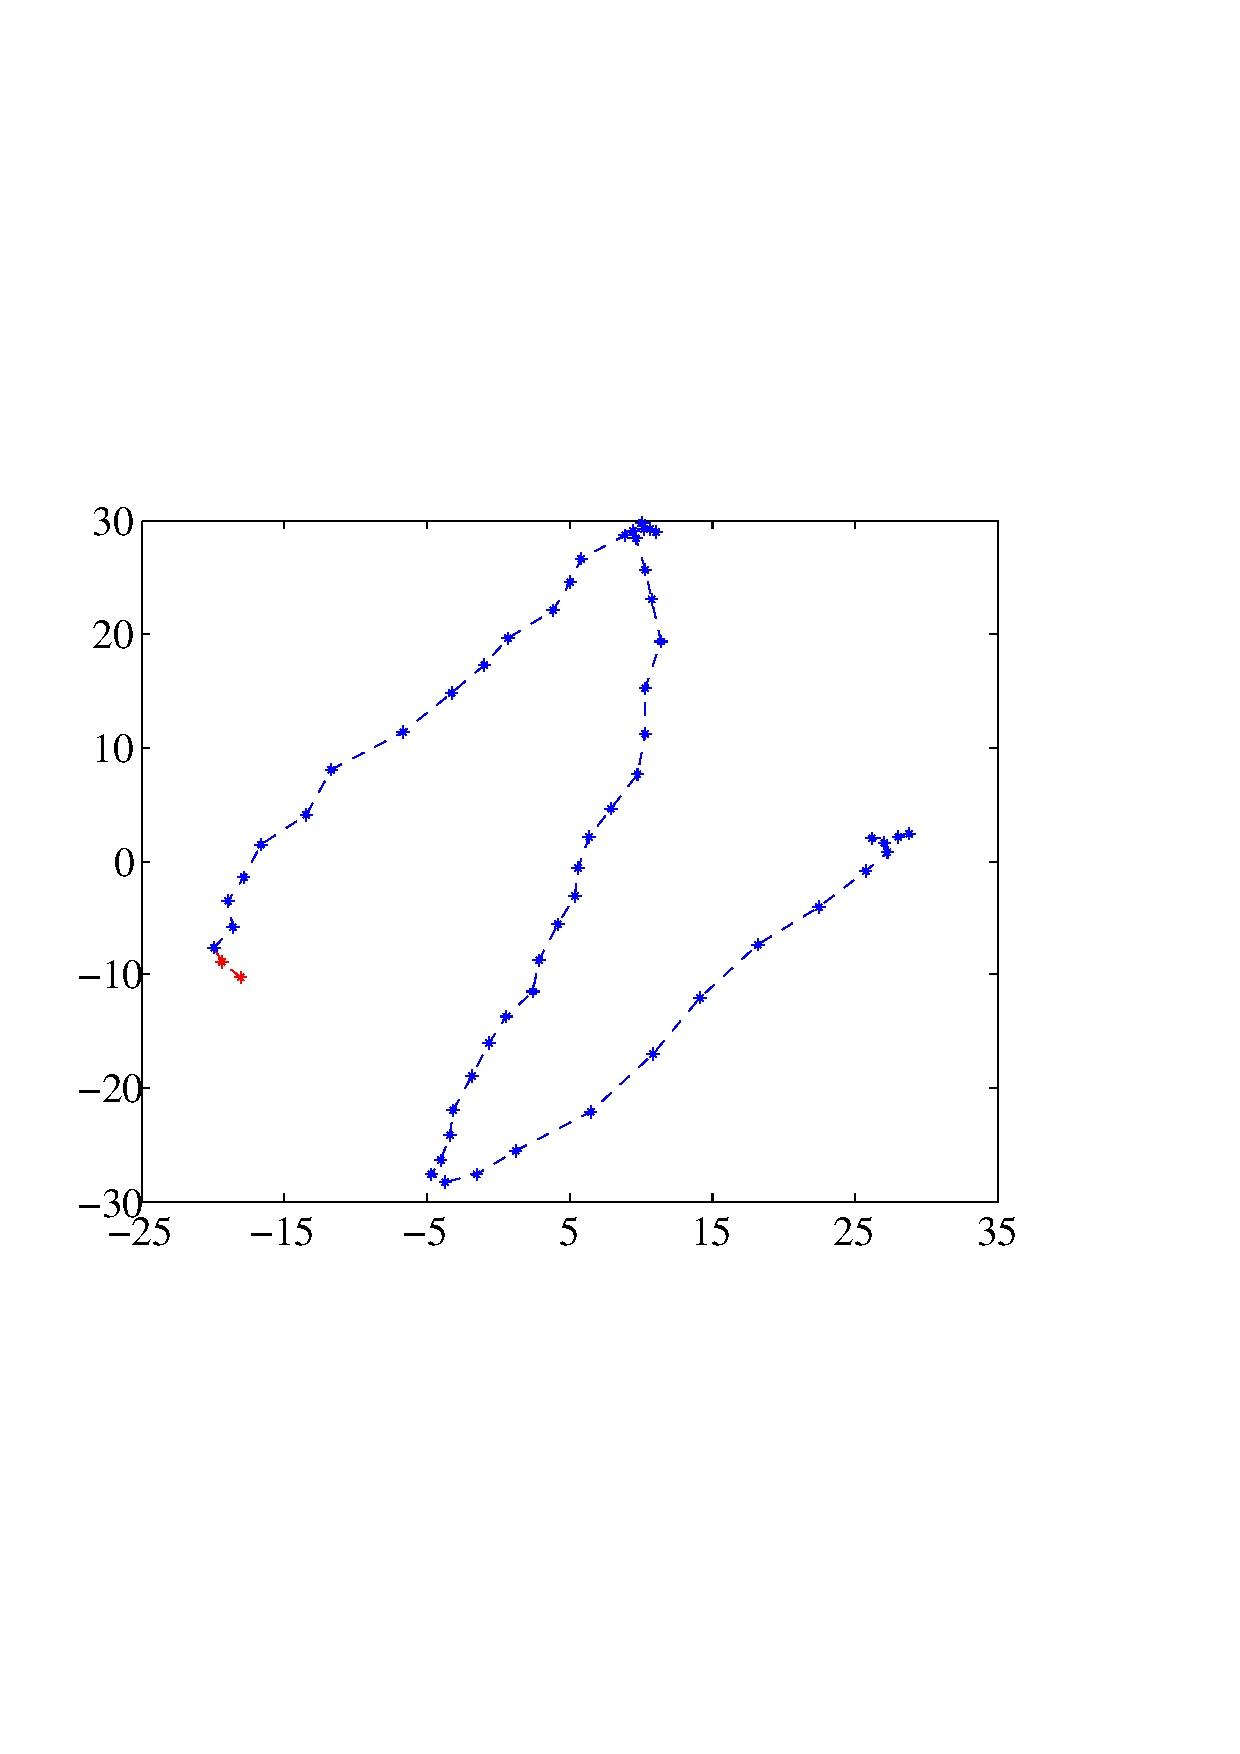
\includegraphics[width=\textwidth]{fig/distance-2m.pdf}\\
                \centering  (a)
                \end{minipage}
            }
            \hfill
            \subfigure{
                \begin{minipage}[b]{0.23\textwidth}
                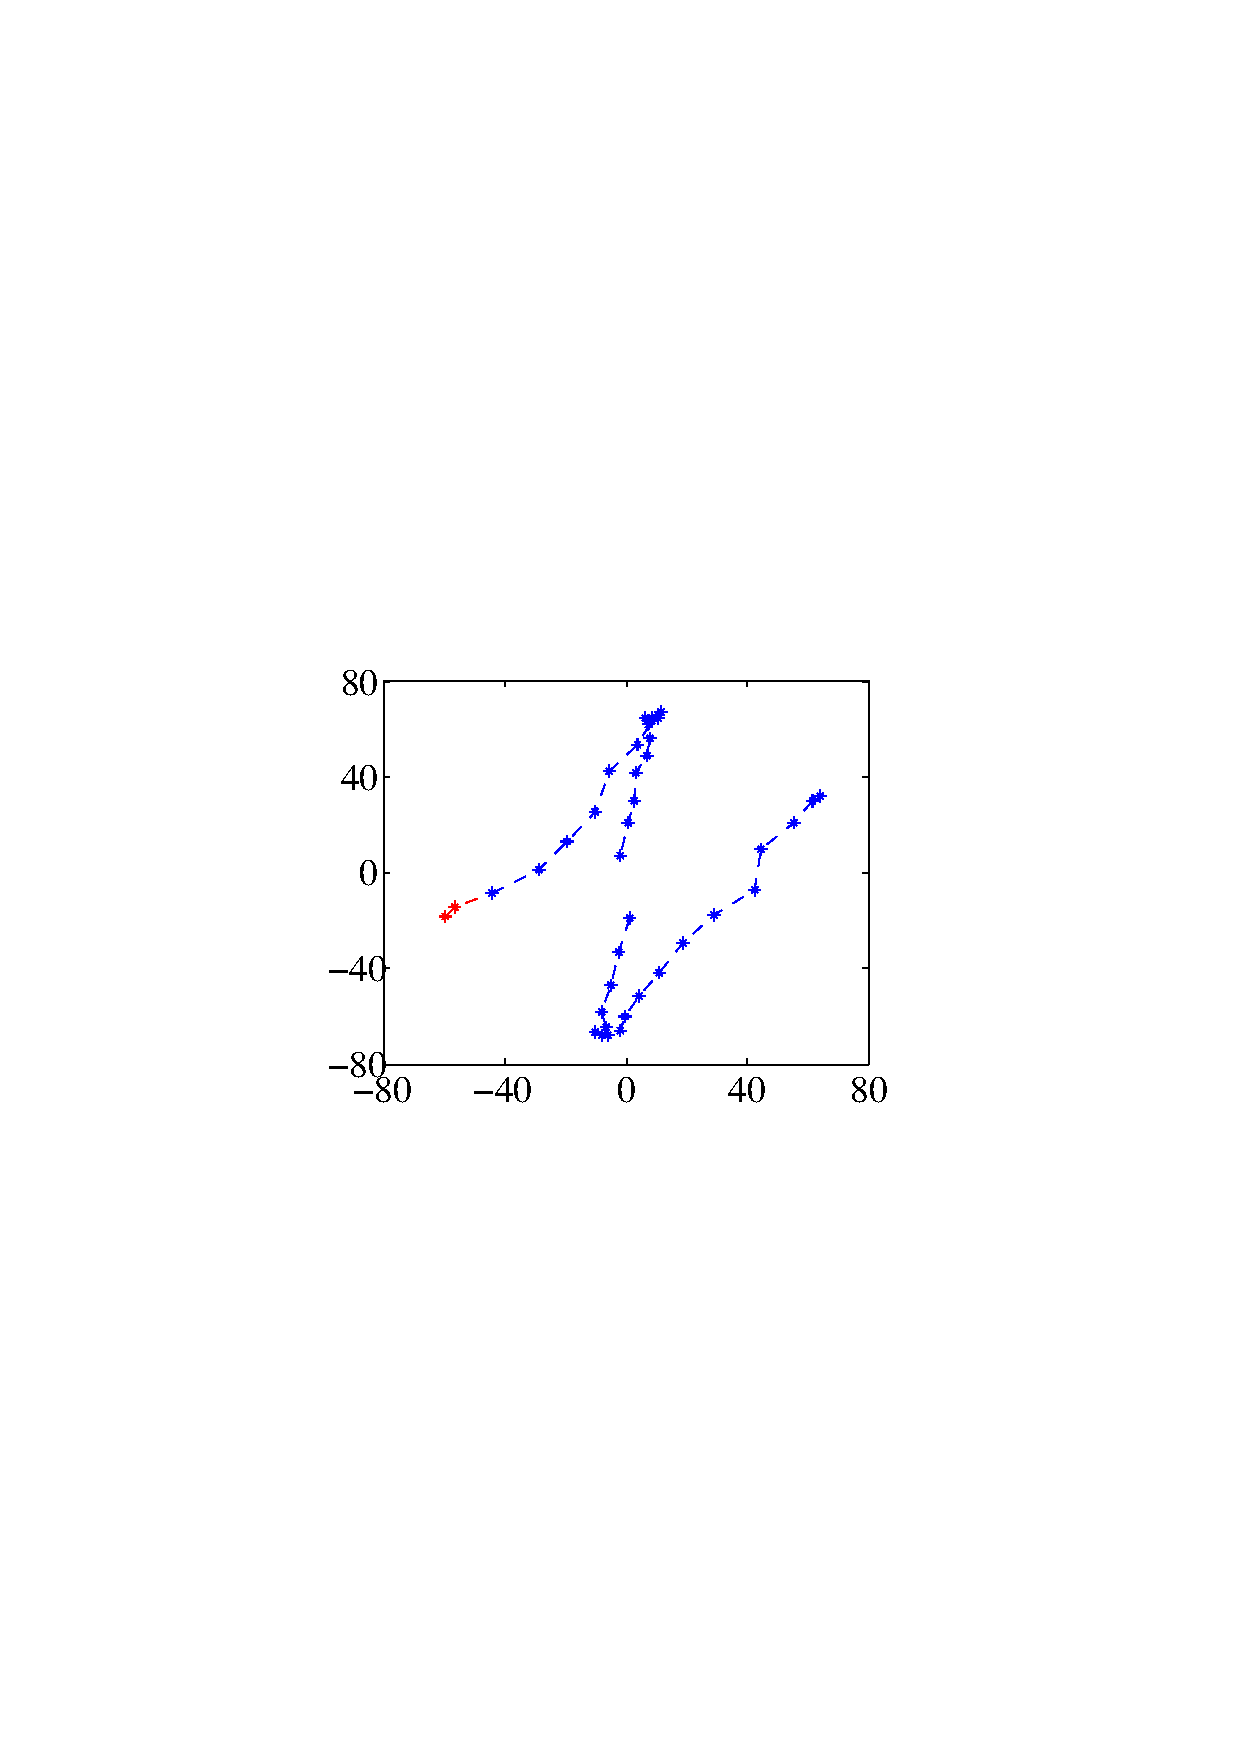
\includegraphics[width=\textwidth]{fig/distance-3m.pdf}\\
                \centering  (b)
                \end{minipage}
            }
            \hfill
            \subfigure{
                \begin{minipage}[b]{0.23\textwidth}
                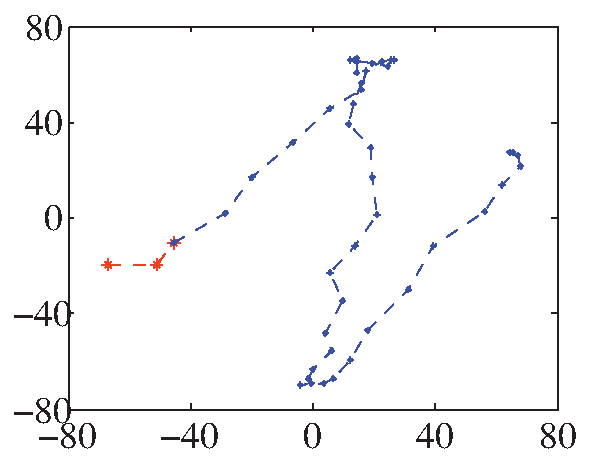
\includegraphics[width=\textwidth]{fig/distance-3-5m.pdf}\\
                \centering  (c)
                \end{minipage}
            }
            \hfill
            \subfigure{
                \begin{minipage}[b]{0.19\textwidth}
                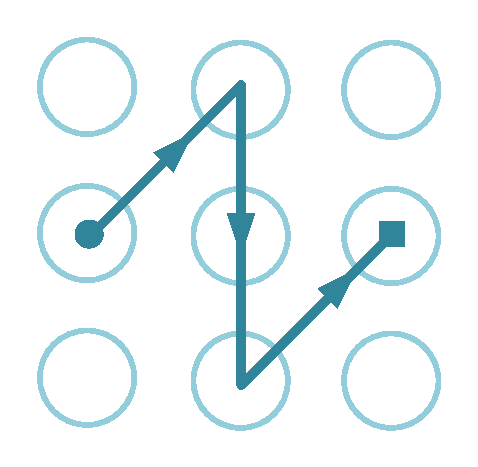
\includegraphics[width=\textwidth]{fig/distance-pattern.pdf}\\
                \centering  (d)
                \end{minipage}
            }

            \caption{Tracked fingertip trajectories (user's perspective) for the pattern shown in (d) from a video filmed from a distance of 2m (a), 3m (b), and 3.5m (c) respectively away from the target device. The tracking quality decreases when the filming distance is greater than 3m. }
            \label{fig:distance-show}
        \end{figure*}

       \subsubsection{Evaluation using alternative security metric}
       \label{sec:eval_gussingp}
        In addition to using the complexity metric defined by Equation~\ref{equ:compscore}, we also evaluate our attack
        based on how likely a pattern will be used by users.  For this purpose, we use the
        guessing probability  proposed in~\cite{Heidt2016Refining}. This metric measures the pattern's strength by
        considering how likely a pattern is to be guessed. The guessing probability is the likelihood estimation from
        the hidden Markov model trained on collected, real-world data~\cite{uellenbeck2013quantifying}. The larger the
        likelihood, the more likely the pattern would have been
        selected by a user.  We choose this metric because a similar security metric
        based on statistical analysis of real-world passwords haven been widely used in prior studies of text-based
        passwords~\cite{Kelley:2012:GAM:2310656.2310715,Bonneau:2012:SGA:2310656.2310721}.

        %Intuitively, if an attacker is to guess the pattern, he would start from a candidate pattern with the
        %largest guessing probability (because that pattern is most likely to be used by users).
        %Therefore, the probability can be use as a proxy for categorizing how frequent a pattern would be used by ordinary users.


          To translate the guessing probability to a frequency score, we first sort all the 120 testing patterns used
          in this experiment in ascending order, based on their guessing probabilities. By doing so, patterns with a
          higher probability (i.e. more commonly used patterns) will appear after those with a lower probability (less commonly
          used patterns) on the sorted list. Next, we give each pattern a numeric number (termed \emph{guessing number}), starting from 1 for
          the first pattern of the sorted list, and we increase the number by 1 as we move down to next (more commonly used) pattern on the sorted list. We then use the following
          formula to calculate the frequency score, $f_{P}$, of a pattern, $P$:

        \begin{equation}
            f_{P}=\log_{10} {G_P}
            \label{equ:guessing_number}
        \end{equation}
        where $G_P$ is the guessing number of pattern $P$.


            Less commonly used patterns have a smaller guessing number and thus will have a lower frequency score using Equation~\ref{equ:guessing_number}. With
            this metric in place, we divide our 120 patterns collected from our participants into three groups:
            \emph{low}, \emph{median} and \emph{high}. Patterns in the \emph{high} group are more likely to be used by users than the patterns in the
            \emph{low} group. The \emph{high} group has a value of less than 4.2, the \emph{median} group
            has a score between 4.2 and 5.1, and the \emph{low} group must have a score greater than 5.1.
            Using this partition strategy, each group has around 40 patterns.

        \begin{figure}[t!]
            \centering
            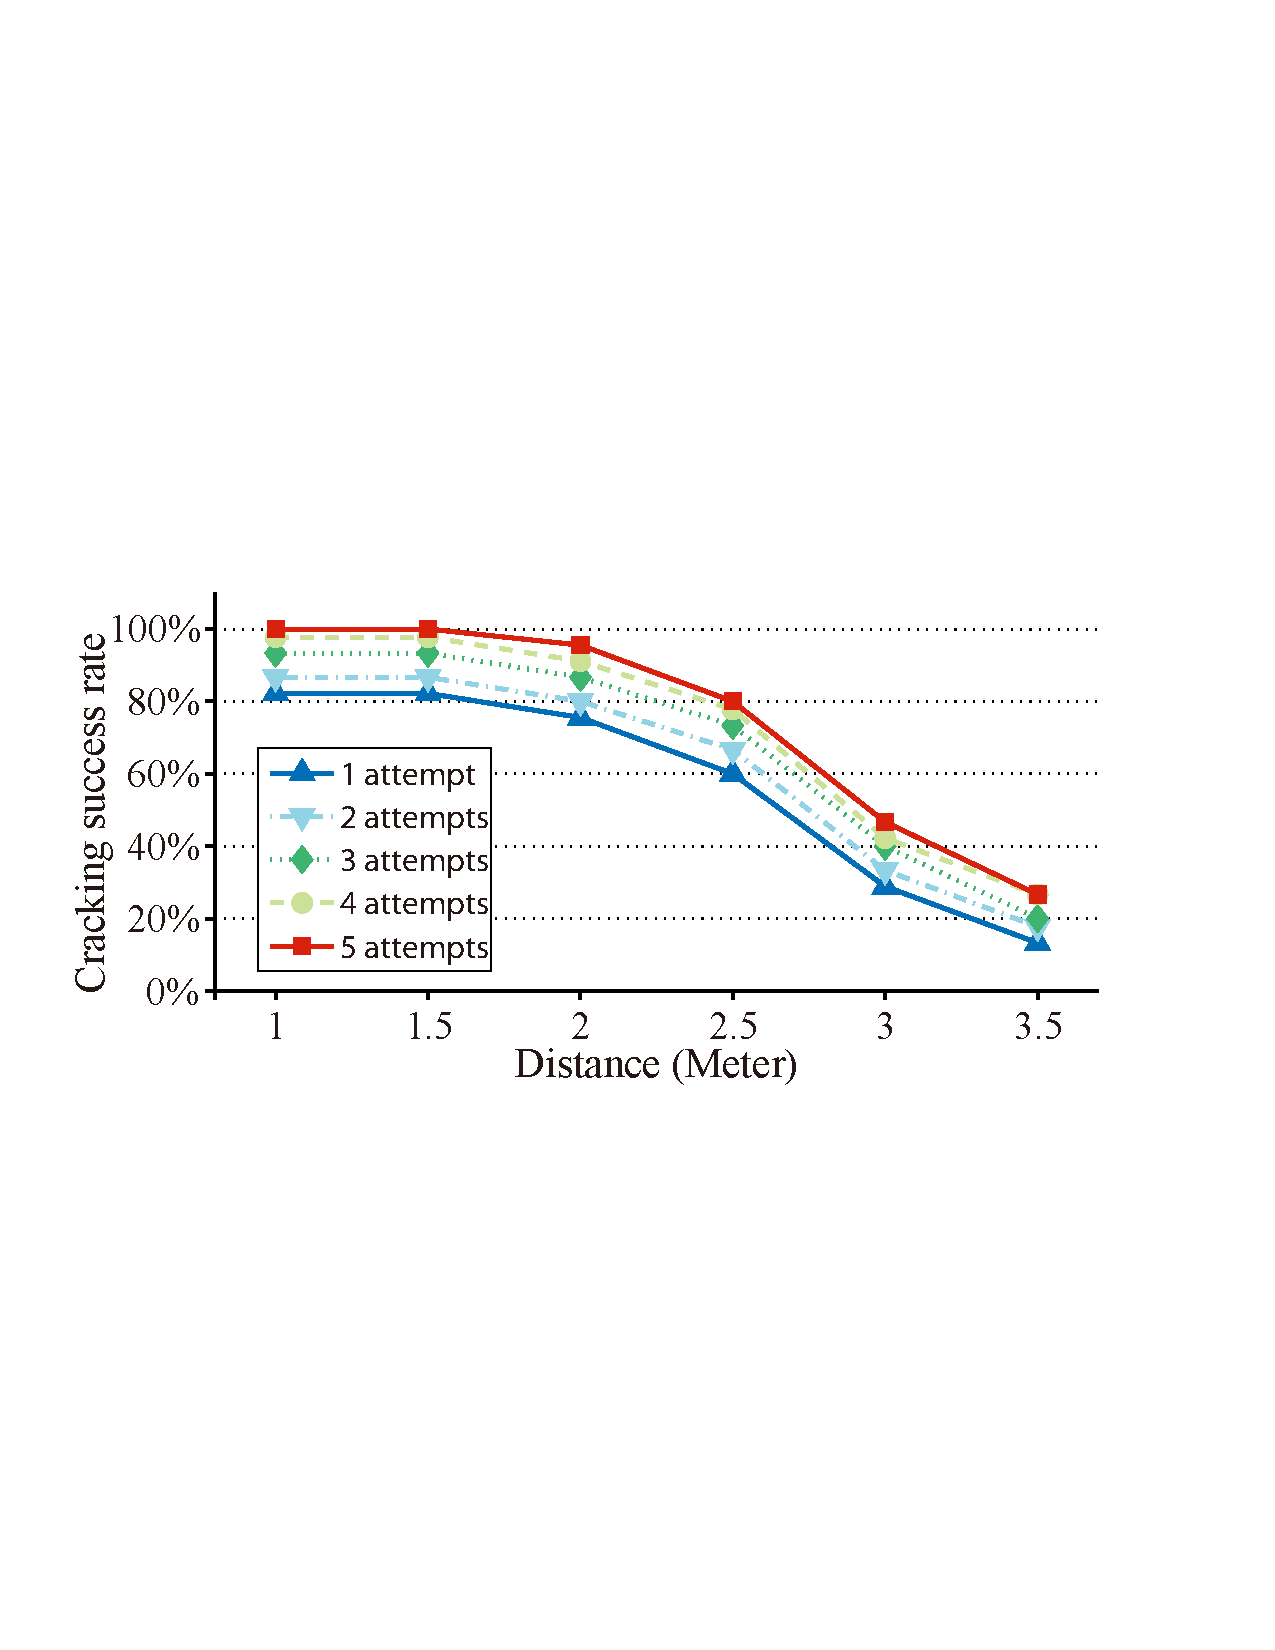
\includegraphics[width=0.5\textwidth]{fig/12.pdf}
            \caption{Impact of the filming distance.}
            \label{fig:fig12}
        \end{figure}

            \FIXED{Intuitively, the simple pattern that is classified by Equation~\ref{equ:compscore} is likely to belong to the high group that is classified by Equation~\ref{equ:guessing_number}. Likewise, the median and complex patterns are likely to respectively belong to the median and low group.  However, the fact is that the two partition strategies are different. To prove this, we stat the number of the patterns both belonging to the simple and high group, median and median group and complex and low group. Then we figure out the repetition rate of each two group. Table~\ref{tab:repetition_rate} shows the repetition rate of each two groups. It presents that many patterns are different under the two partition strategy which indicates that the two partition strategies are different.}

            Figure~\ref{fig:usage-crackingNum} illustrates the cracking success rate for different categories under
            numbers of attempts.  As can be seen from the diagram, the success rate with one attempt for the patterns
            in the \emph{high} group is 42.5\%. This success rate is lower than patterns in other groups. This is because that
            the patterns in the \emph{high} frequently used group are typically simple and symmetry patterns, for which our tracking algorithm produces more
            than one candidate pattern. This is in line with our observation using the complexity metric defined in
            Equation~\ref{equ:compscore}. Nonetheless, our attack can successfully crack over 90\% of the pattern of
            each group. This confirms that the video-side channel is a real threat for the Android locking pattern.

    \subsection{Impact of Filming Distances \label{sec:distances}}

\begin{figure}[t!]
    \centering
    \vspace{0.1cm}
    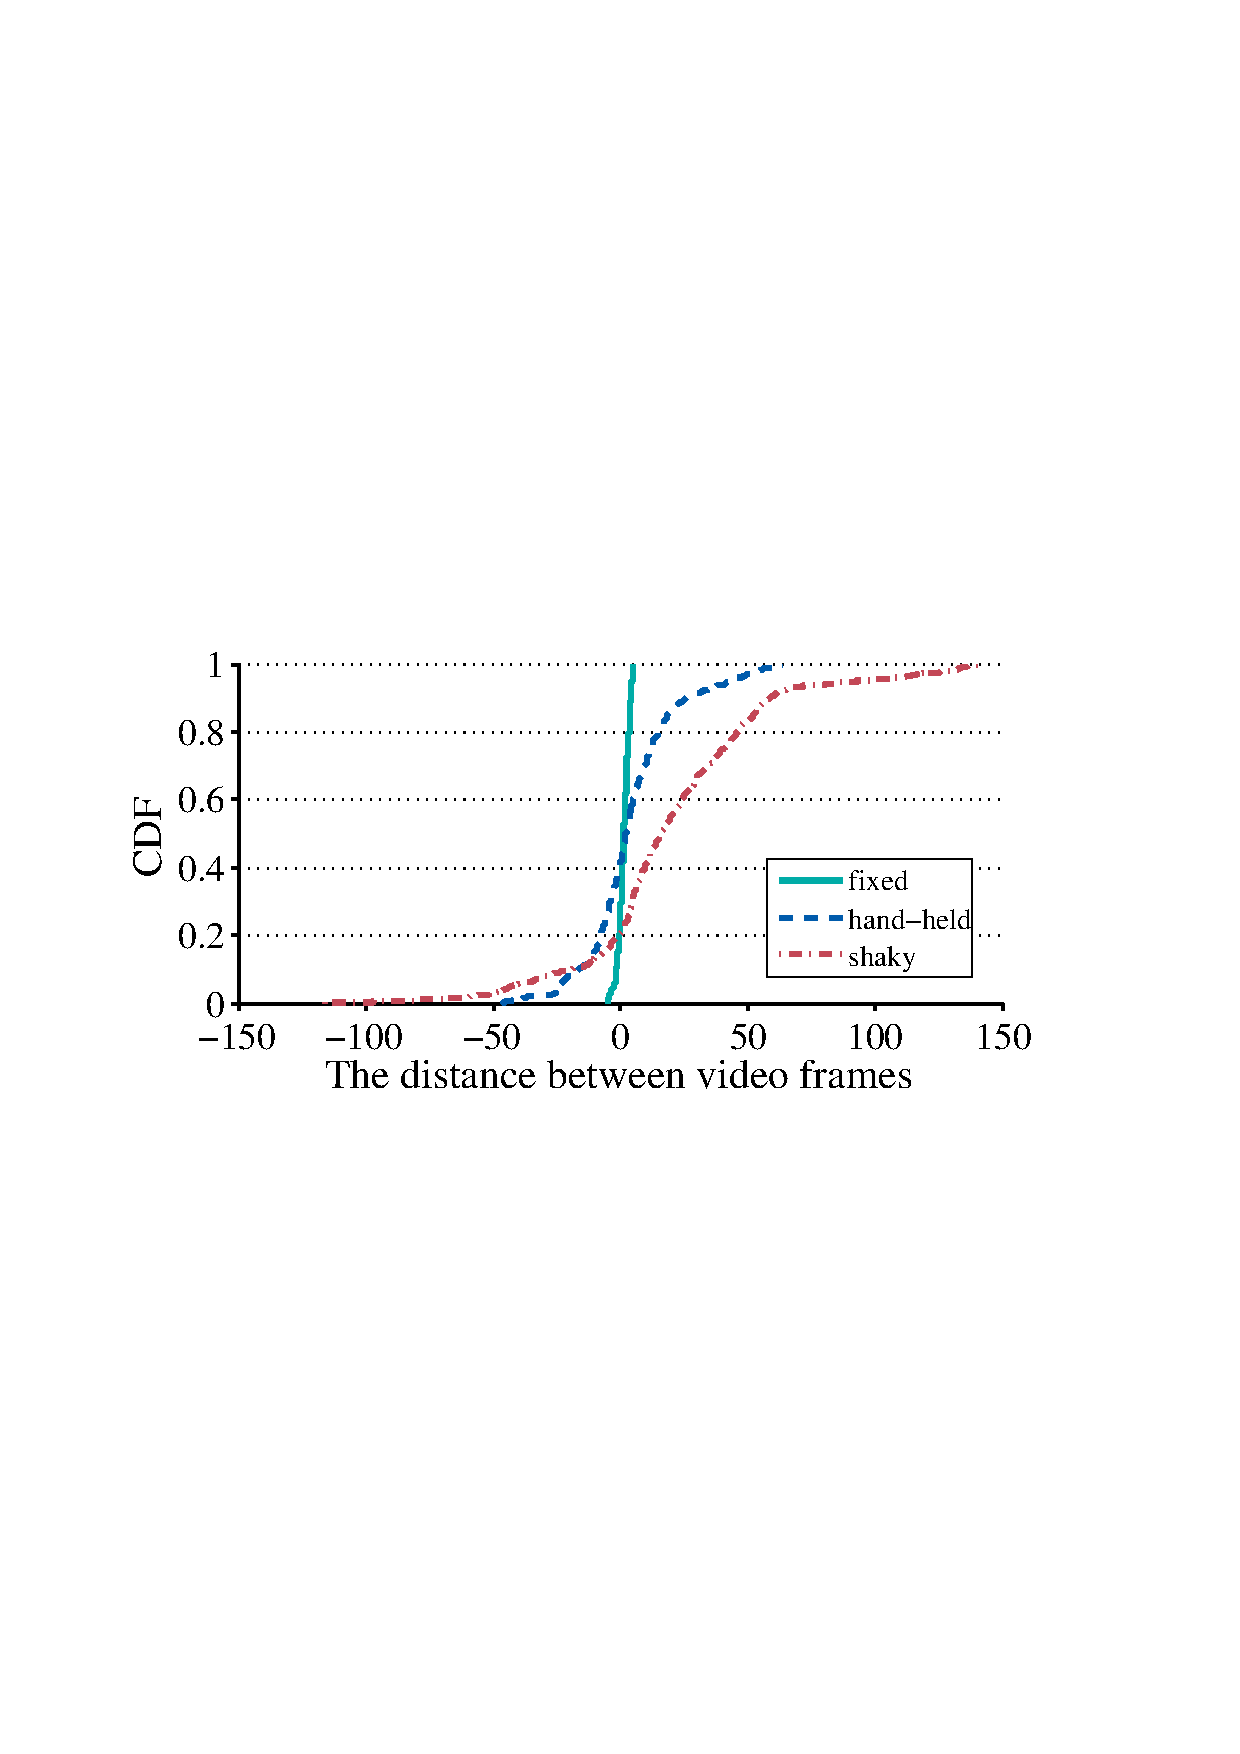
\includegraphics[width=0.5\textwidth]{fig/13.pdf}
    \caption{The cumulative distribution function (CDF) for different video recording modes.}
    \label{fig:fig13}
\end{figure}

\begin{figure}[!t]
    \centering
    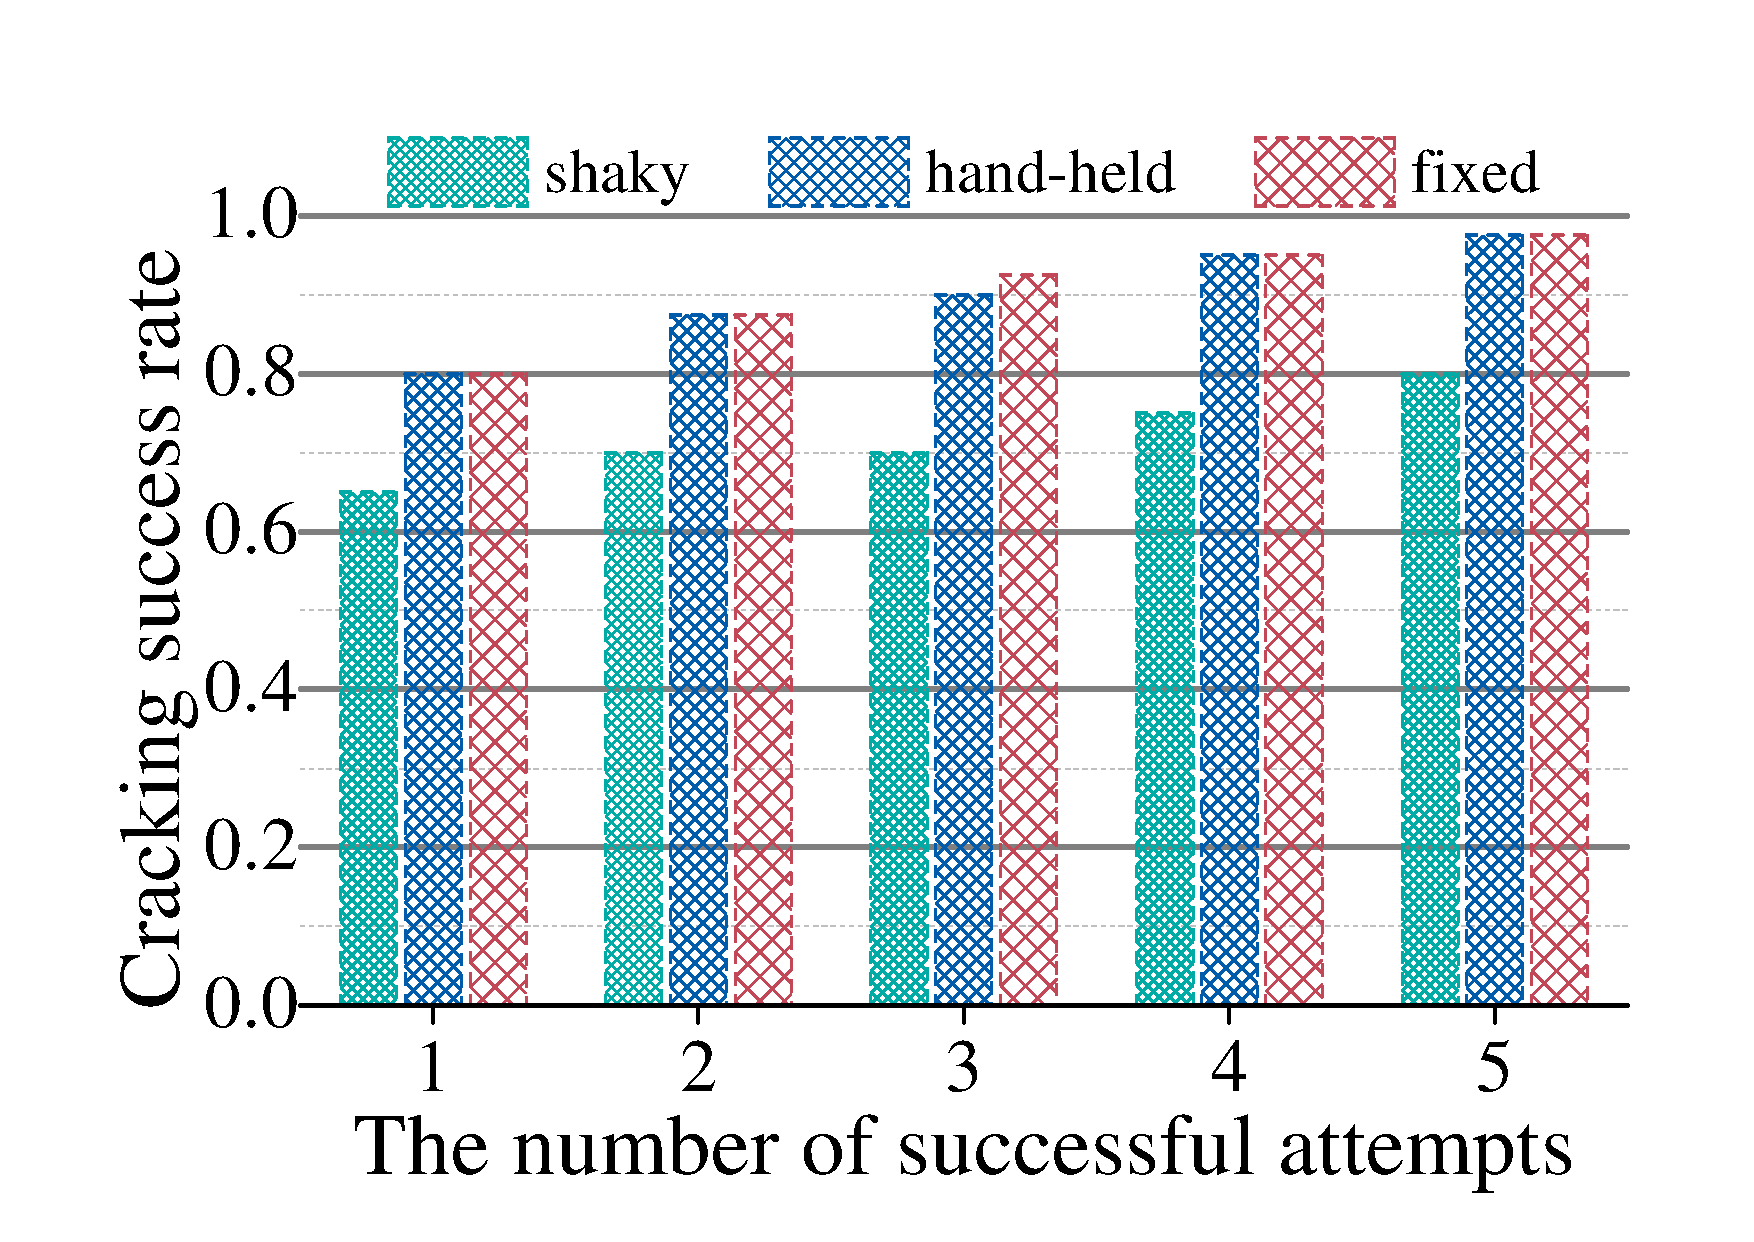
\includegraphics[width=0.5\textwidth]{fig/14.pdf}
    \caption{Impact of camera shake. Our approach has the same success rate under the hand-held and the fixed modes and the performance degradation under the shaky mode is modest. }
    %\FIXME{We should evaluate this on 3 and 4 attempts.}
    \label{fig:fig14}
\end{figure}

        \noindent \textbf{Result 2:} \emph{We can crack over 80\% of the patterns in five attempts, if the video was filmed using a smartphone within a distance of 2.5 meters away from the target.}

           We would like to know how the filming distance affects the
           success rate of the attack. To do so, we used all the 120 collected patterns and we varied the
           filming distance from 1 meter to 3.5 meters.
           Figure~\ref{fig:fig12} shows how the cracking success rate changes
           as the filming distance increases. There are minor discrepancies in the success rate between this diagram and Figure~\ref{fig:fig10}
            because we used less patterns in this experiment.
           When the filming distance is less than 2 meters, our approach can crack all patterns in five attempts.
           The success rate drops significantly when
           the filming distance is greater than 2.5 meters.
           Beyond this point, the quality of the video filmed by a mobile phone tends to drop significantly with many object deformations. The degradation of the video quality makes it difficult for the TLD algorithm to successfully track objects across video frames.
            This is confirmed by Table~\ref{tab:tab1}
           which shows that the tracking precision for the fingertip and the device edge drops from around 99\% to
           68\% when the filming
           distance increases from 2 meters to 3.5 meters. The increased
           tracking failures result in an increased number of missing
           points on the tracked trajectory, leading to a deteriorative performance in identifying candidate patterns.
           This can be seen from Figure~\ref{fig:distance-show} where the quality
           of tracking clearly decreases when the filming distance is greater
           than 3 meters.
           Nonetheless, our approach can
           achieve a high success rate when the filming distance is within
           2.5 meters. Such a distance allows an attacker to
           record the video without raising suspicions in many day-to-day scenarios (some of these are
           depicted in Figure~\ref{fig:fig1}).

            We also evaluated our approach on videos filmed using an entry-level
            single-lens reflex (SLR) camera, Nikon D90, with a low-end 105mm lens. The SLR camera
            was placed from a distance of 9 meters away from the target
            device. For this set of videos, we are able to achieve the same
            performance when compared to using videos filmed by a mobile
            phone camera with a 2-meter filming distance. The further filming
            distance is largely due to better video quality brought by the advanced
            SLR camera and the lens. Therefore, in practice, an attacker can
            also use a professional video recording device to launch the
            attack from a further distance.

        \begin{figure}[t!]
            \centering
            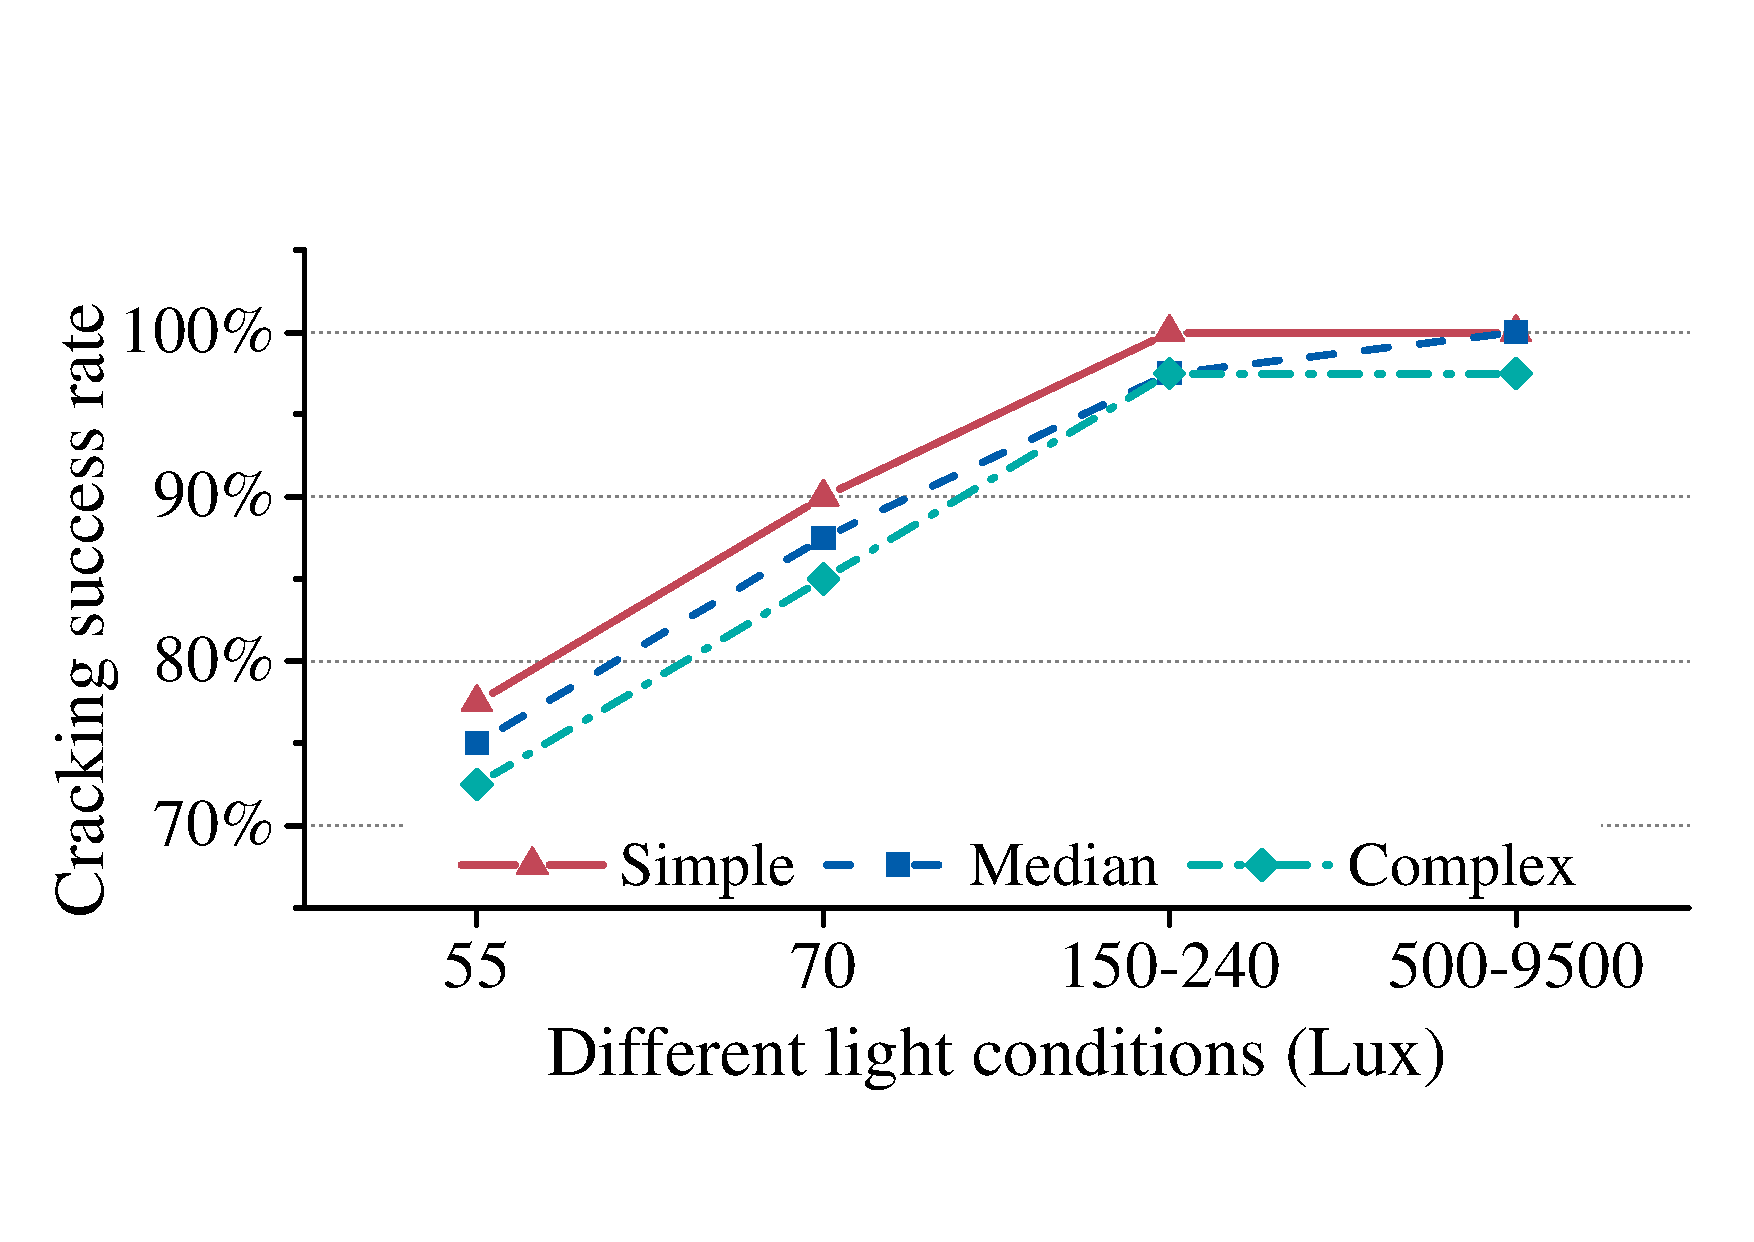
\includegraphics[width=0.5\textwidth]{fig/light.pdf}
            \caption{The cracking success rate within five attempts under different lighting conditions.}
            \label{fig:light}
        \end{figure}

        \begin{table}[!t]
            \centering
            \caption{Tracking precision vs filming distance}
            \vspace{-0.2mm}
            \label{tab:tab1}
            \small
            \begin{tabular}{ccccc}
                \toprule
                \textbf{Distance}& 1 m & 2 m & 3 m & 3.5 m \\
                \midrule
                \textbf{fingertip}  & 100\% & 98.7\% & 80.9\% & 68\% \\
                \textbf{device edge} & 100\% & 99.4\% & 90.6\% & 69\% \\
                \bottomrule
            \end{tabular}
        \end{table}

    \subsection{Impact of Camera Shake}

    \noindent \textbf{Result 3:} \emph{Our method can tolerate a certain degree of camera shake in the hand-held mode.}

    In this experiment, we used an IPhone4S smartphone to record how a pattern is drawn on a Huawei Honor7 phone. This experiment was carried out under three settings:
    \emph{fixed}, \emph{hand-held} and \emph{shaky}, where the filming
    device was respectively fixed using a tripod, hand-held, and hand-held but with constant movements of
     approximate 2cm in the horizontal or the vertical directions. The recording device was placed on the left-front, front, and right-front of the target device.
    In the experiment, we affixed the target device on a table using double-sided tapes.



    We use a reference point to quantify camera shake. The point
    is the center position of an area of the target device. The area is marked by a boundary box on the first
    frame (see Figure~\ref{fig:fig5}). We calculate the difference (in terms of pixels) for where the
    reference point was seen in two consecutive video frames. We then use the difference to measure the degree of camera shake.
    Figure~\ref{fig:fig13} shows the cumulative distribution function (CDF)
    of camera shake under the three different filming settings.
    Here, the wider the distribution is, the less steady the
     filming is. The shaky mode is least stable where the difference of the reference point between two video frames can be up to 250 pixels.


    Figure~\ref{fig:fig14} shows that our approach has the same performance under
    the hand-held and the fixed modes. The modest camera sake under the hand-held mode
    has little impact on performance thanks to our camera-shake calibration method. We observe deteriorative performance
    under the shaky mode, but the performance degradation is modest (80\% vs 97\%
    in 5 attempts). In reality, an attacker would avoid drastic
    camera shake by firmly holding the video recording device.

     \begin{figure}[!t]
        \centering
        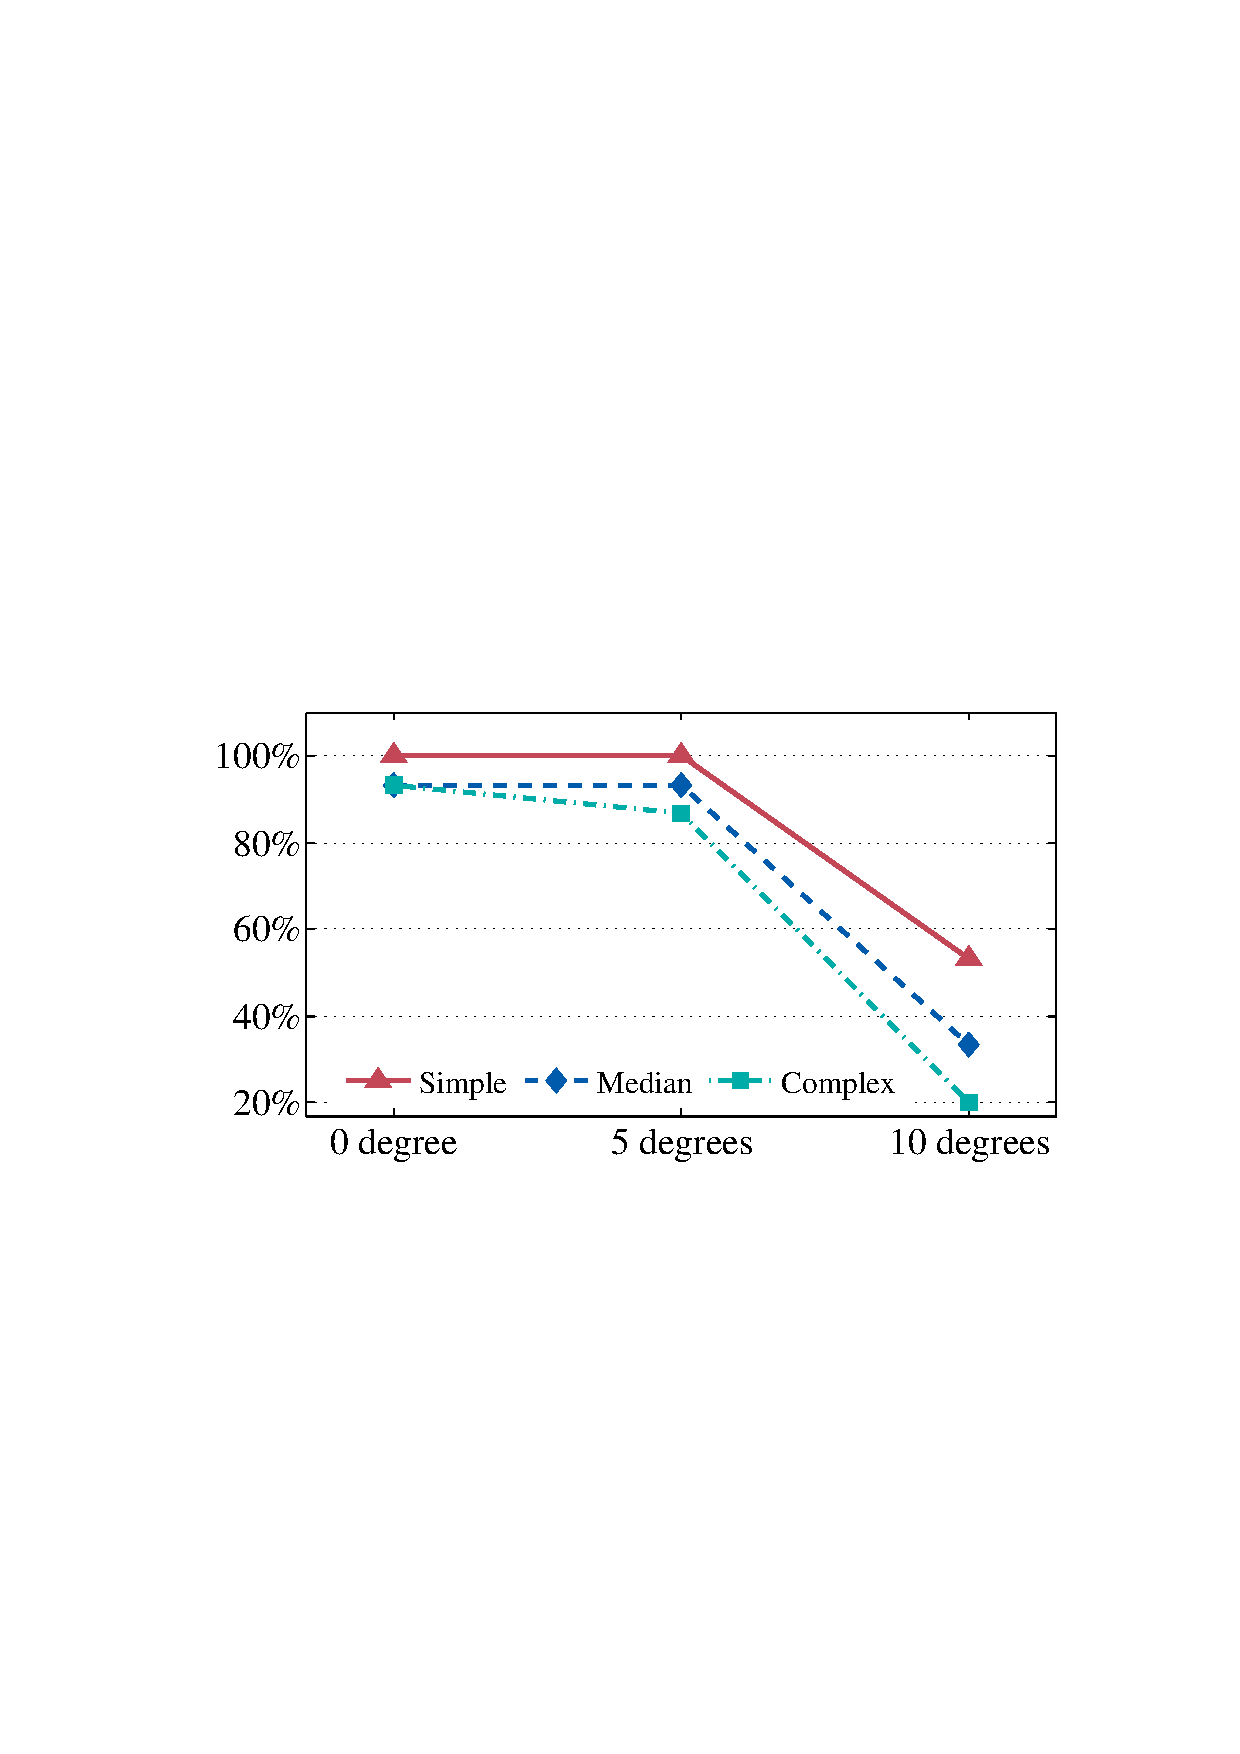
\includegraphics[width=0.5\textwidth]{fig/15.pdf}
        \caption{Impact of estimation errors of filming angles.}
        \label{fig:fig15}
    \end{figure}


    \subsection{Impact of Lighting Conditions \label{sec:light}}
    \noindent \textbf{Result 4:} \emph{Low-light has a negative impact on the success rate of the attack but our approach can still break over 70\% of the patterns when the video was filmed in a low-light environment.}

    In this experiment, videos were recorded under different lighting conditions both indoor and outdoor.
    The experimental settings are given in  Table~\ref{tab:light}.
    The light intensity of these conditions range from 9500
    lux (strong light), onto 240 lux (normal light), and 55-70 lux (low light).
    These represent some of the day-to-day scenarios where filming can
    take place. For each setting, we tested all the 120 patterns on a Xiaomi MI4 phone and used
    an iPhone4S phone to record the video. The filming camera was placed on the
    left-front, front, and the right-front of the target device from a distance
    of 2 meters.


    Figure~\ref{fig:light} shows that the success rate increases when video filming was performed in a brighter lighting condition as the light intensity
    changes from 55 lux to 9500 lux. This is expected as low-light leads to
    increased video noise, blurred motions and poor focus, which all have a
    negative impact on the TLD algorithm. Nonetheless, our attack
    can still crack over 70\% of the patterns in a filming
    environment of low light.

       \begin{table}[!t]
            \centering
            \caption{Lighting Conditions}
            \label{tab:light}
            \scriptsize
            \begin{tabular}{lcccc}
                \toprule
                \textbf{Scenarios} & Indoor  & Indoor & Indoor  & Outdoor\\
                \midrule
                \textbf{Time} & nighttime &  nighttime & daytime & daytime \\
                \textbf{Light Source}& warm LED & white fluorescent & sunlight &  sunlight \\
                \textbf{Light Intensity (Lux)} & $55-70$ & $70-100$ & $150$--$240$ & $500$--$9500$ \\
                \bottomrule
            \end{tabular}
        \end{table}


    \begin{table}[!t]
            \centering
            \caption{Screen sizes per target phone}
            \label{tab:screen-size}
            \scriptsize
            \begin{tabular}{cccc}
                \toprule
                \textbf{Screen-size}& \textbf{IPhone4S }& \textbf{Honor7} & \textbf{Samsung Tablet} \\
                \midrule
                Height(cm)$\times$Width(cm) & $11.5\times5.9$ & $14.3\times7.2$ & $24.2\times15.0$ \\
                \bottomrule
            \end{tabular}
            %\vspace{-4mm}
    \end{table}

    \begin{table}[!t]
            \centering
            \caption{Filming camera parameters}
            \label{tab:camera-parameters}
            \small
            \begin{tabular}{lrrrr}
                \toprule
                \textbf{Parameters}& \textbf{IPhone6} & \textbf{Vivo X7} & \textbf{MI4} & \textbf{Note4} \\
                \midrule
                Frame Rate (fps) & $30$ & $30$& $30$ & 30 \\
                Pixels & 8mp & 13mp & 13mp & 16mp \\
                Focus (mm) & 4.15 & 4 & 4 & 4.2 \\
                Sensitivity (ISO) & 3200 & 3200 & 3000 & 5000 \\
                \bottomrule
            \end{tabular}
    \end{table}

    \subsection{Impact of Filming Angle Estimation \label{sec:angle}}

    \noindent \textbf{Result 5:} \emph{Our attack performs well when the error of filming angle estimation is less than 5 degrees.}

   Recall that our attack needs to transform the fingertip movement trajectory to the
   user's perspective based on an estimation of the filming angle
   (Section~\ref{sec:transformation}).
   Because our filming angle estimation
    algorithm gives highly accurate results, we did not find the estimation error to be an issue in our experiments.
   Nonetheless, it is worth studying how the estimation error affects the success rate of our attack. To do so, we deliberately added an error of 5-10 degrees to the estimation in this experiment.

    Figure~\ref{fig:fig15} shows the results of this experiment. When the error is less than $\pm 5$ degrees, there is little impact
    on \emph{complex} patterns and no impact at all on \emph{simple} and
    \emph{median} patterns. However, an estimation error of more than 10 degrees can significantly affect the success rate.
    Given such errors, the resulting trajectory after transformations will
    be significant different from the correct pattern.
    For example, when the estimation error is 10 degrees from the
    true value,  on average, 0.8, 2.6 and 4.2 line segments per pattern respectively will
    be incorrectly labelled for \emph{simple}, \emph{median} and
    \emph{complex} patterns. This explains why the success rate for complex patterns drops significantly when the filming angle estimation error is greater or equal to 10 degrees.

   \begin{figure}[!t]
        \centering
        \subfigure{
             \begin{minipage}[t]{0.5\textwidth}
                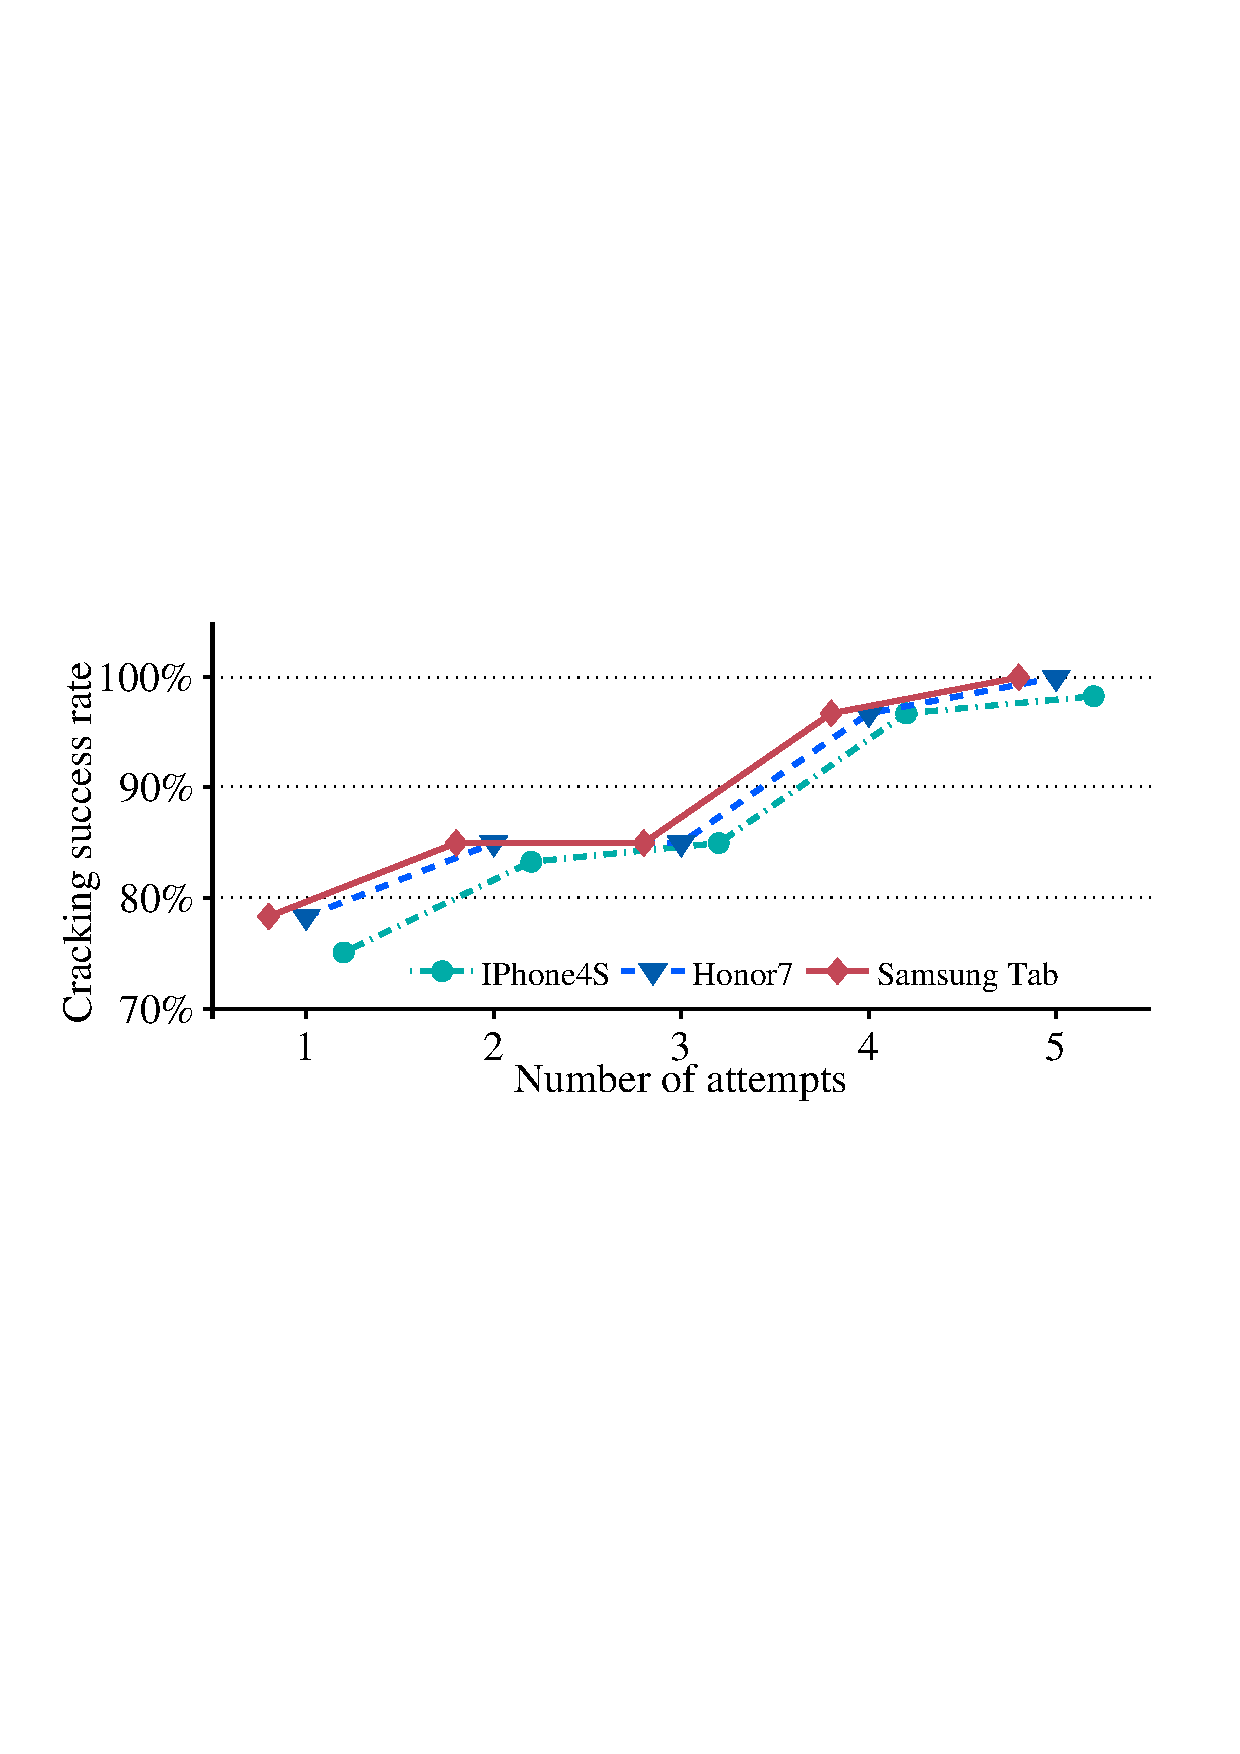
\includegraphics[width=\textwidth]{fig/screen_size.pdf}\\
                \centering  (a) screen size
             \end{minipage}
        }
        \subfigure{
             \begin{minipage}[t]{0.5\textwidth}
                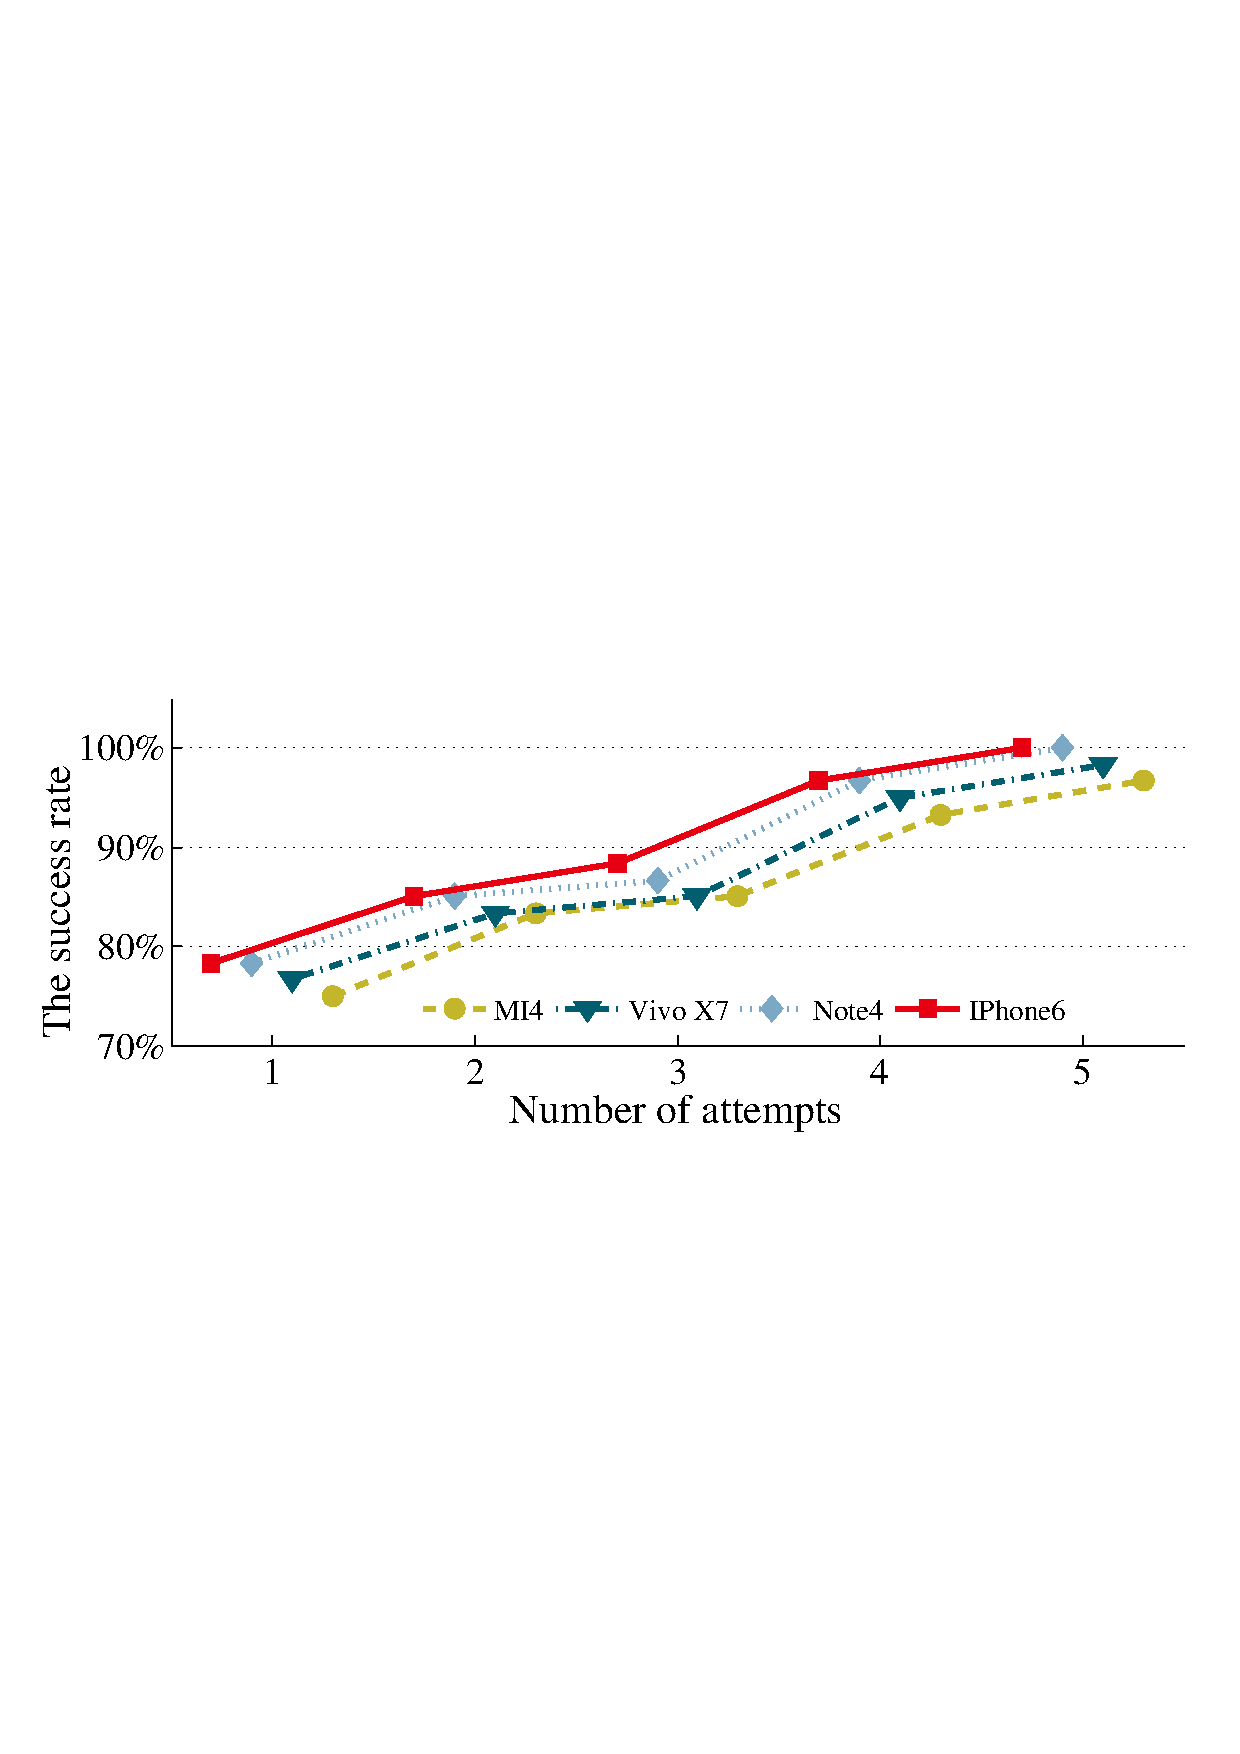
\includegraphics[width=\textwidth]{fig/camera_brands.pdf}\\
                \centering  (b) camera brands
             \end{minipage}
        }
        \caption{The cracking success rate for different target screen sizes and filming cameras. }
        \label{fig:screen_size}
    \end{figure}

        \begin{figure*}[!t]
            \centering
            \subfigure{
                \begin{minipage}[t]{0.45\textwidth}
                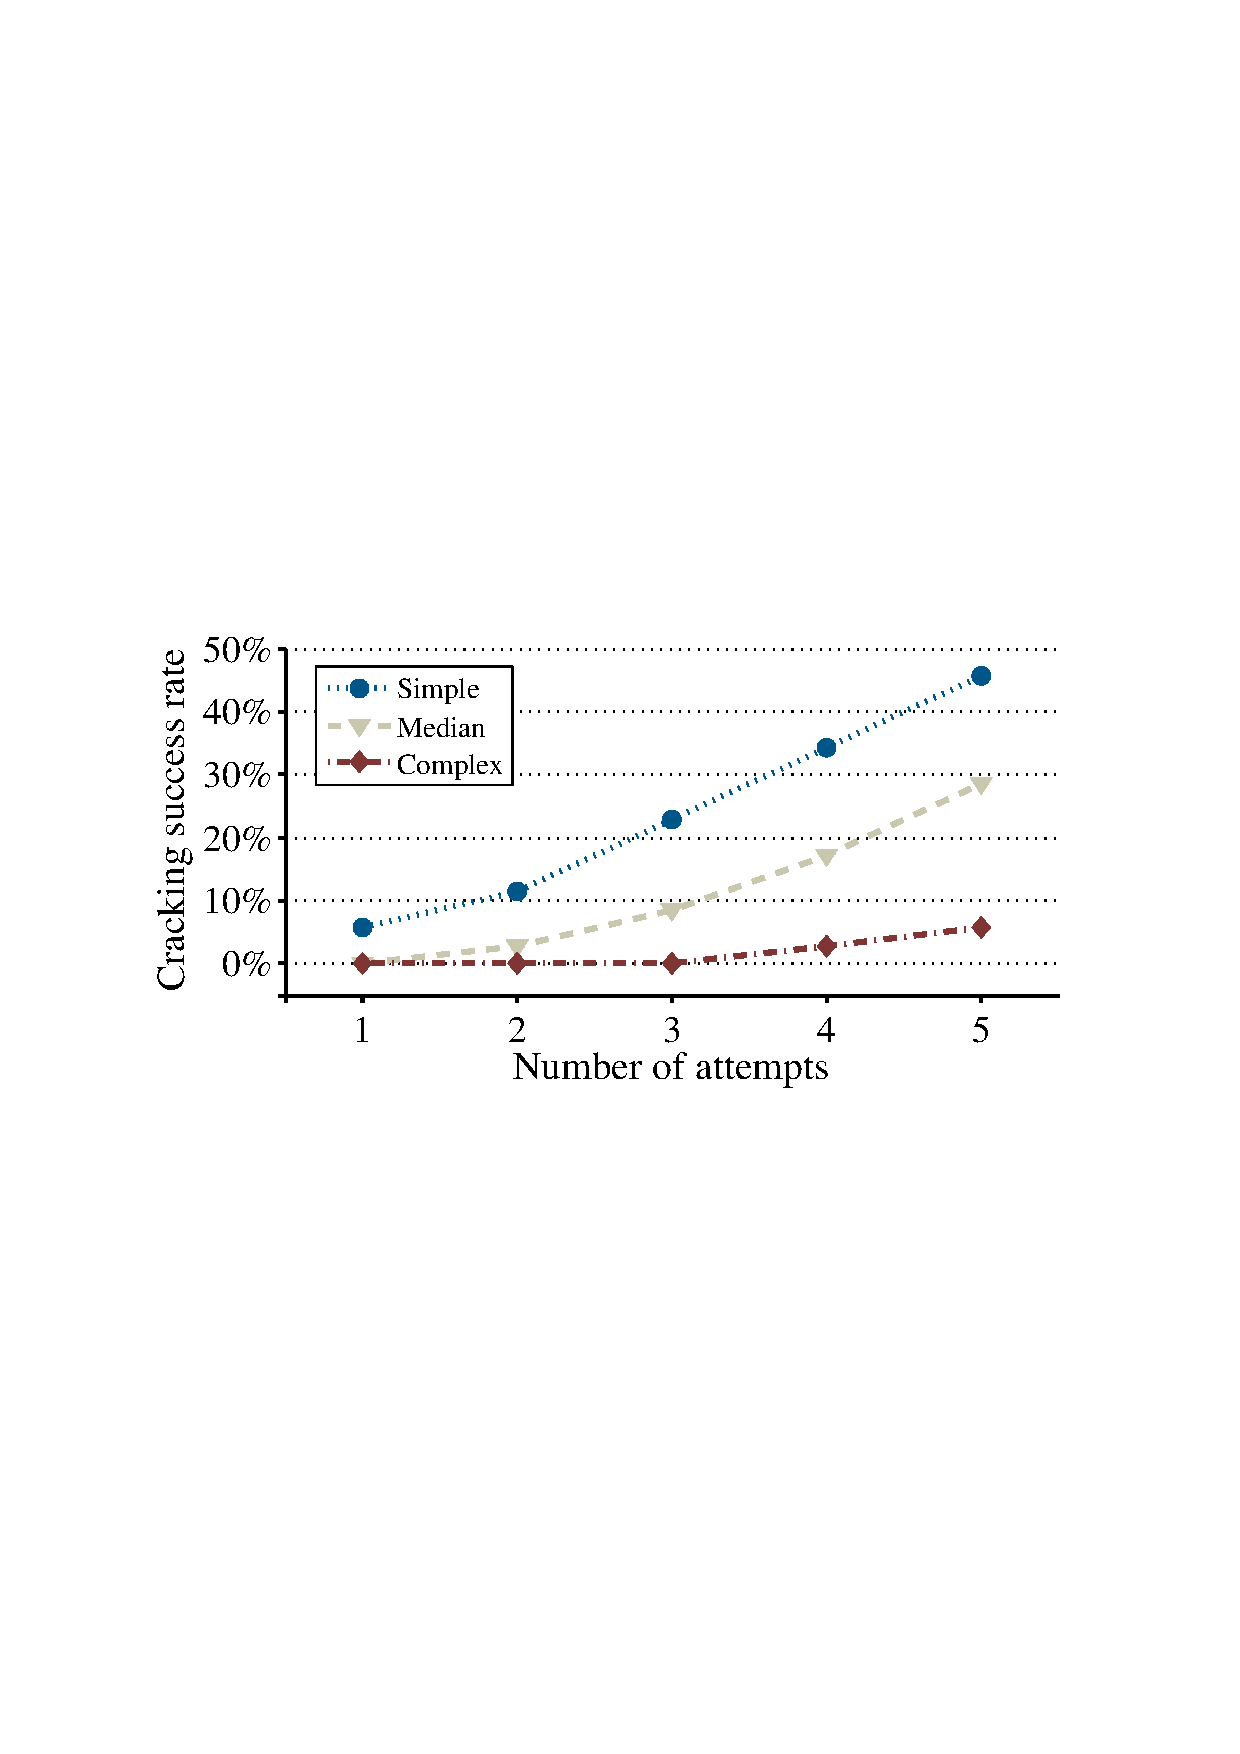
\includegraphics[width=\textwidth]{fig/look-video.pdf}\\
                \centering  (a) video watching
                \end{minipage}
            }
            \hspace{0.2cm}
            \subfigure{
                \begin{minipage}[t]{0.45\textwidth}
                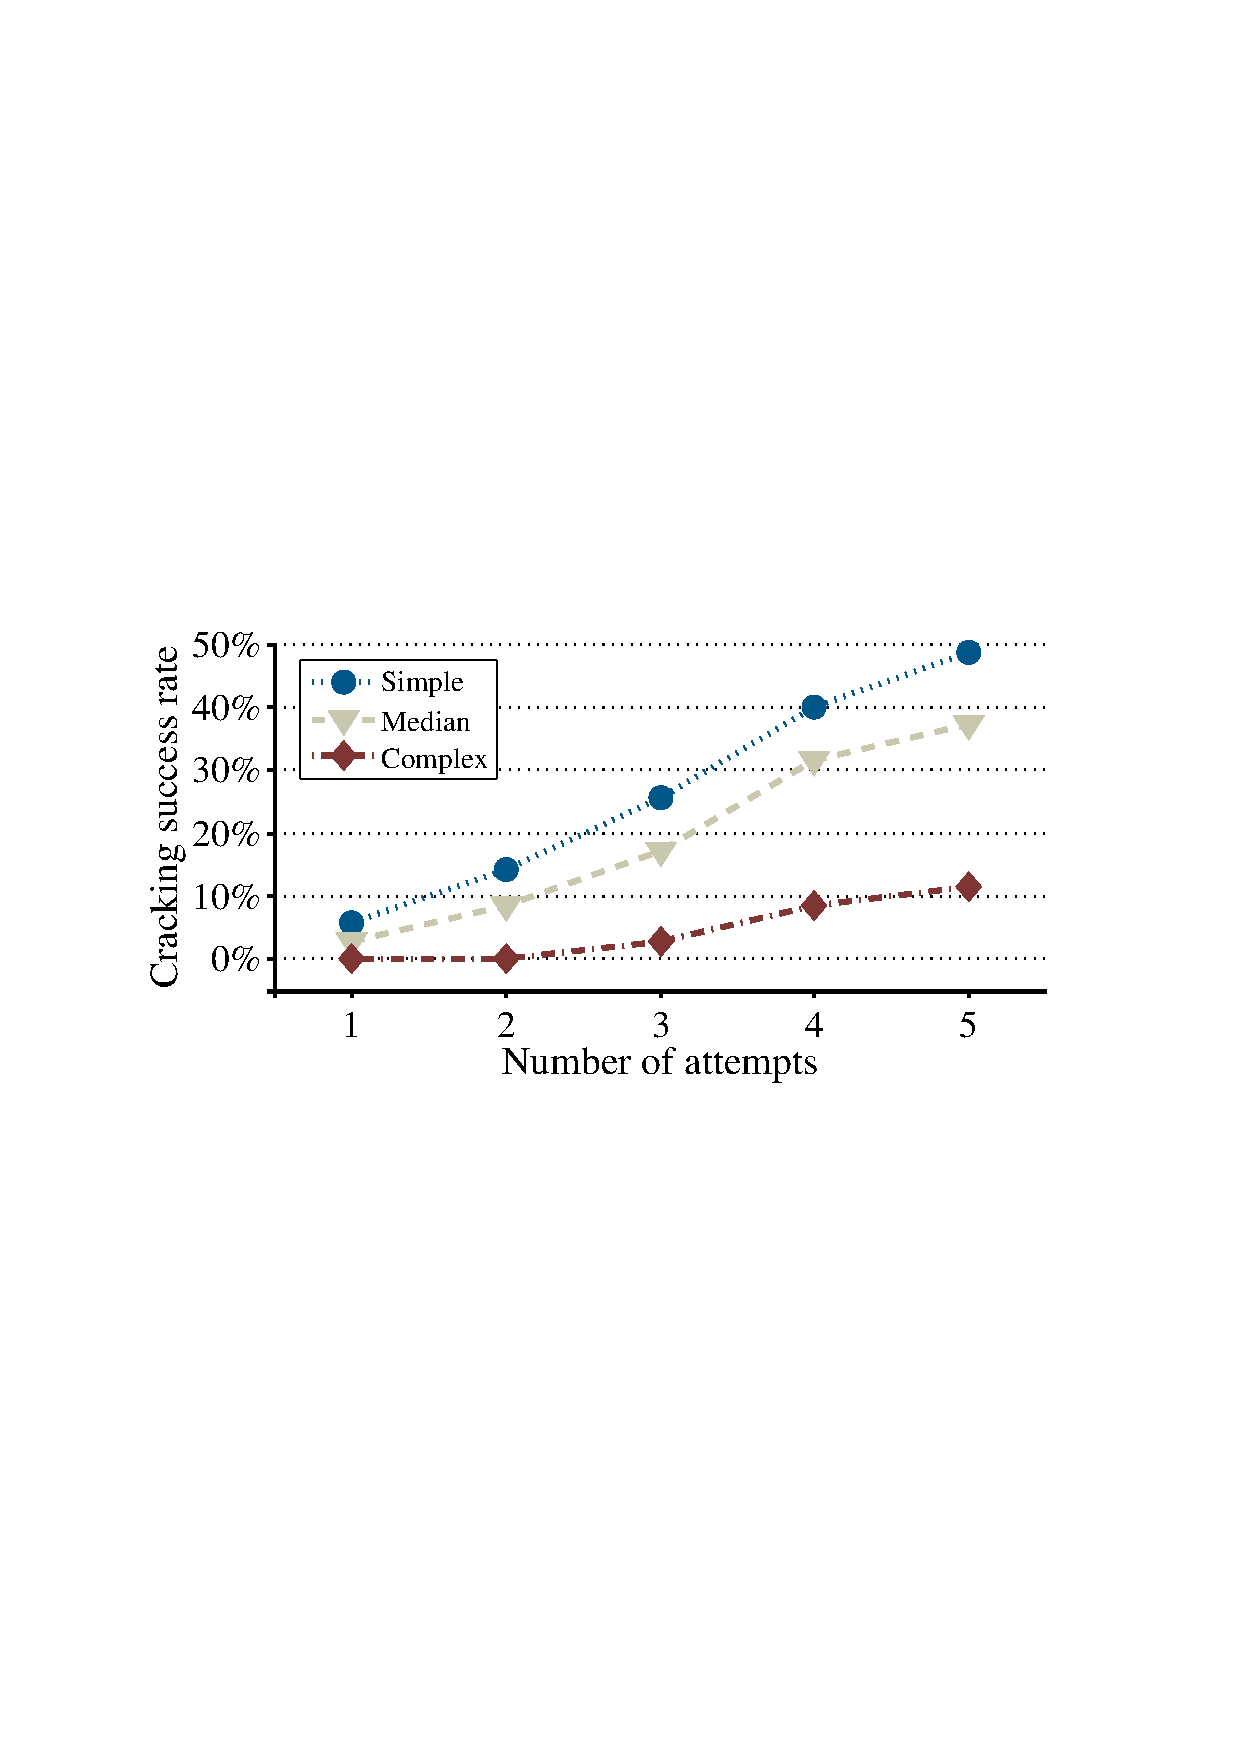
\includegraphics[width=\textwidth]{fig/look-finger.pdf}\\
                \centering  (b) direct observations
                \end{minipage}
            }
            \vspace{-2mm}
            \caption{Success rates of guessing patterns through watching the video (a) or direct observations (b).}
            \label{fig:look-unlocking process}
        \end{figure*}

    \subsection{Impact of Screen Sizes and Cameras}
    \label{section: screen-size and cameras}
    \noindent \textbf{Result 6:} \emph{The size of the smartphone touch-screen and the mobile camera have little impact on the success rate.}

    Intuitively, the success of the attack would be influenced by the size of
    the touch-screen because the physical length of the pattern depends on
    the size of the screen. Likewise, the accuracy also may be affected by
    the quality of the video because of the filming camera. To evaluate this
    effect, we asked 10 participants to randomly select 90 patterns (30
    patterns from each of the three pattern categories). We used four
    recording devices: IPhone6, Xiaomi MI4, Vivo X7 and Samsung Note4 to
    record the video footage. The target devices are a Huawei Honor7, a
    Samsung Galaxy Tablet, and an IPhone4S\footnote{For iOS, participants are asked
    to draw  patterns on the login interface of Alipay as iOS
    currently does not support pattern lock natively.}. The filming distance is 2
    meters from target device. Table~\ref{tab:screen-size} gives the screen
    size of each device, which ranges from 3.5 \emph{inch} (IPhone4S) to
    9.6 \emph{inch} (Samsung Tablet). Table~\ref{tab:camera-parameters} lists
    the mobile cameras and their main performance parameters, which
    represent some of the most commonly used smartphone cameras.

    Figure~\ref{fig:screen_size} (a) confirms that our attacking method
    is not significantly affected by the size of the
     target device's screen. Our approach achieves a 98.3\%  success rate within five
    attempts when the screen size is 3.5 \emph{inch} (a small screen in the current
     mobile market). It can crack all tested pattern locks when
    the size of screen is larger than 5.2 \emph{inch} (Honor7). We also
    evaluated  our approach using different types of filming cameras.
    The result is presented in Figure~\ref{fig:screen_size}
    (b). Our method can reconstruct all patterns (100\%) within five trials using
    the IPhone6 and the Note4 because their camera settings (hardware and software) lead to a better video
    quality.   When using MI4 and Vivo X7 for filming,
     the success rate can reach 96.7\% and 98.9\% within five
    attempts respectively, where our approach incorrectly identifies 3 and 1 (out of
    90) patterns respectively due to blur motion in the video footage.
    This experiment shows that the screen size and filming camera
    have little impact on the attacking success rate.

    \subsection{Inferring Patterns with Eyes}

    \noindent \textbf{Result 7:} \emph{Our attacking methodology significantly outperforms direct observation techniques.}

   In this experiment, we investigate whether an attacker can infer the pattern by
   simply watching the video or through direct observations. To answer this question, we asked each of our 10 participants to watch 60 videos (where
   a pattern was drawn by other participants) to guess the pattern.  We
    only played the video segment during which a pattern is drawn to the participant (around 3 seconds per video).
   To familiarize participants with the process, we
    played  five sample videos and showed the correct patterns at the end of each video to our participants before the experiment.
   Each participant then had 10 minutes to watch a video and five chances to guess a pattern. They could adjust the playing speed and
   replay the video multiple times as they wished.

        \begin{figure}[!t]
            \centering
            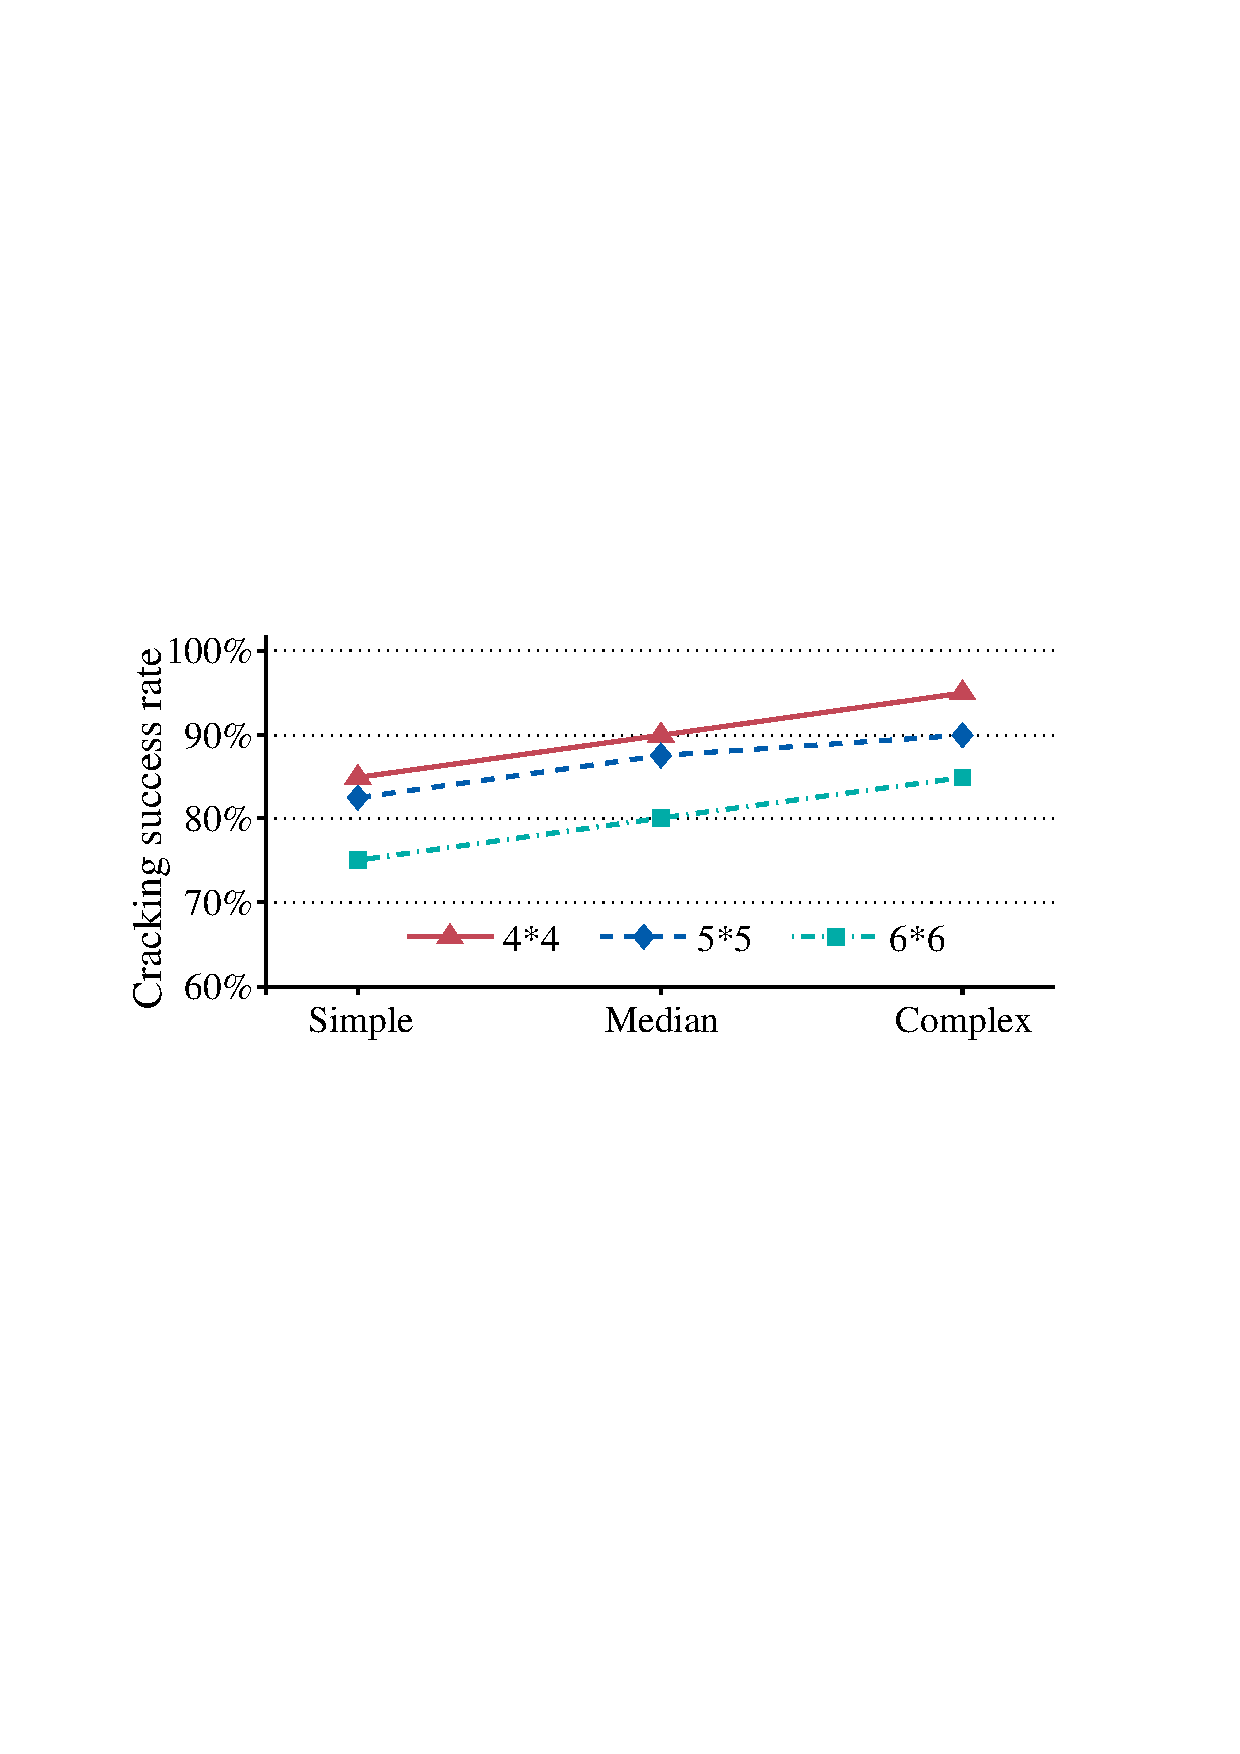
\includegraphics[width=0.45\textwidth]{fig/scalability.pdf}
            \caption{Success rates of our attack for different locking grids.}
            \label{fig:scalability}
        \end{figure}

        Figure~\ref{fig:look-unlocking process} (a) shows the success rate of pattern guessing with
        bare eyes. Our participants correctly guessed for nearly half of the
        simple patterns in five attempts. However, they found that it is difficult
        to infer complex patterns with many line segments, overlapping lines and intersections.
        The success rate of guessing complex patterns is less than 10\% in five attempts.
        This is not a surprising result
        because although it is possible to correctly guess patterns with
        simple structures by watching the video, doing so for patterns with
        more complex structures is much harder.


    We also asked participants to directly observe how a pattern was drawn
    from a distance of 2 meters away from the target device. The intuition
    behind this evaluation is that human eyes can catch richer information
    over a digital video camera. The results of this experiment are shown in
    Figure~\ref{fig:look-unlocking process} (b).  As can be seen from the
    diagram, although the success rate is improved compared to directly watching the video, the chances for guessing the correct pattern in
    5 attempts are quite low. In
    fact, the success rates are 48.3\%, 38.3\%
    and 11.7\% respectively for simple, median and complex patterns.

    \subsection{Evaluation on Other Pattern Grids\label{sec:scalability}}
    \noindent \textbf{Result 8:} \emph{A pattern grid with more dots provides stronger protection but our attack can still crack most of the patterns.}

        There are a few applications (such as CyanLock) and customized ROMs available to increase the size of the pattern grid from $3\times3$ to $4\times4$, $5\times5$, and $6\times6$.
        Although a $3 \times 3$ grid remains
        a popular choice (as it is supported by the native Android OS), it is worth studying whether
        having more touch dots on a pattern grid leads to stronger security. In this
        experiment, we first ranked all possible patterns for each grid setting in
        ascending order according to their complexity scores. We then equally
        divided the patterns into three groups, simple, medium and complex,
        and asked our participants to randomly select 20 patterns from each group for evaluation. We
        report the success rate of our attack within five attempts. In the experiments, we have adapted our algorithms for each grid setting
        by adjusting the algorithm parameters (such as the line direction numbers).


        Figure~\ref{fig:scalability} shows the success rate of our attack
        for different grids. Similar to a $3 \times 3$ grid, our
        approach achieves a higher success rate for complex patterns over
        simple ones. On average, we can crack 90\% of the complex patterns.
        We observed that a grid with more dots does provide
        stronger protection. For complex patterns, the success rate of our
        attack drops from 95\% on a $4 \times 4$ grid to 87\% on a $6 \times
        6$ grid. For simple patterns, the success rate of our attack drops
        from 85\% on a $4 \times 4$ grid to 75\% on a $6 \times 6$ grid. This
        is because a fingertip trajectory in general could be mapped to a larger number of
        candidates on a grid with more dots. For instance, the pattern shown
        in Figure~\ref{fig:fig2} (f) can be mapped to 55
        candidate patterns on a $6 \times 6$ grid as opposite to 5 on a $3
        \times 3$ grid. Overall, our attack can crack over 75\% (up to 95\%)
        of the patterns within five attempts. One of the purposes of introducing
        pattern grids with more dots is to allow users to use more complex
        patterns. However, this experiment suggests that complex patterns remain less security on
         these grids under our attack.

    \begin{table}[!t]
            \centering
            \caption{PIN-based passwords used in our experiments}
            \label{tab:PIN-based passwords}
            \small
            \begin{tabular}{llllll}
                \toprule
                \textbf{Category} & \multicolumn{5}{l}{\textbf{PIN-based Passwords}}\\
                \midrule
                \rowcolor{gray!10}  & 1234 & 1111 & 1212 & 1004 & 2000 \\
                \rowcolor{gray!10}  & 6969 & 4321 & 1122 & 2001 & 2580 \\
               \rowcolor{gray!10}   \multirow{-3}{*}{Commonly used PINs} & 1357 & 2468 &      &      & \\
                                    & 1205 & 3570 &  0729 & 3719 & 9867 \\
                                    & 5946 & 3451 &  7403 & 2209 & 3560 \\
                                    & 1043 & 4628 & 5372  & 2830 & 7102 \\
               \multirow{-4}{*}{Randomly generated PINs} & 6193 & 2941 & 3471  &      & \\
                \bottomrule
            \end{tabular}
    \end{table}

           \begin{figure}[!t]
            \centering
            \subfigure{
                \begin{minipage}[t]{0.18\textwidth}
                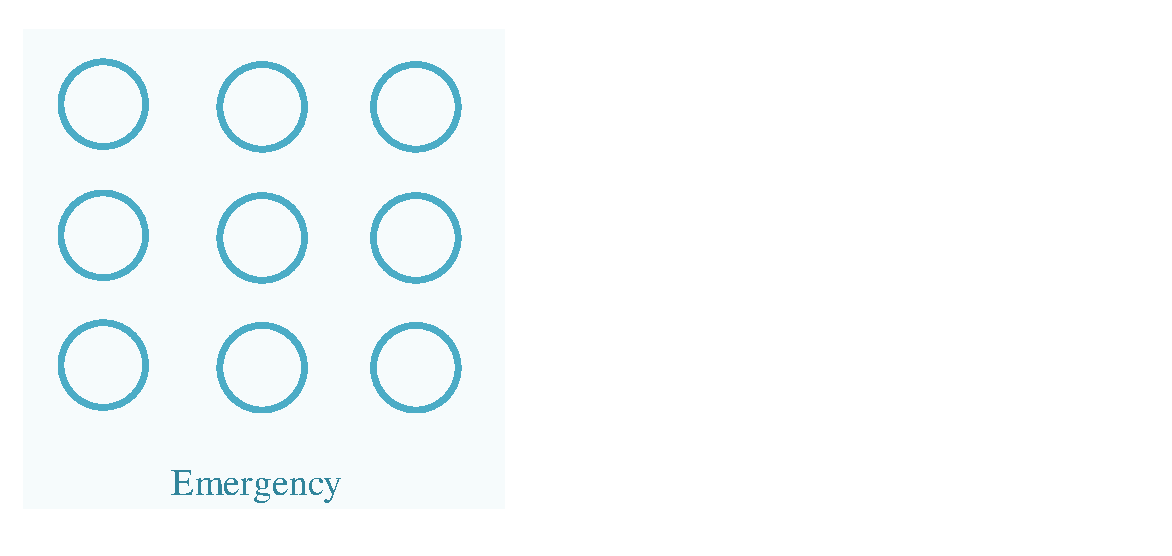
\includegraphics[width=\textwidth]{fig/pattern_screen.pdf}\\
                \centering  (a) pattern-based interface
                \end{minipage}
            }
            \hspace{0.2cm}
            \subfigure{
                \begin{minipage}[t]{0.18\textwidth}
                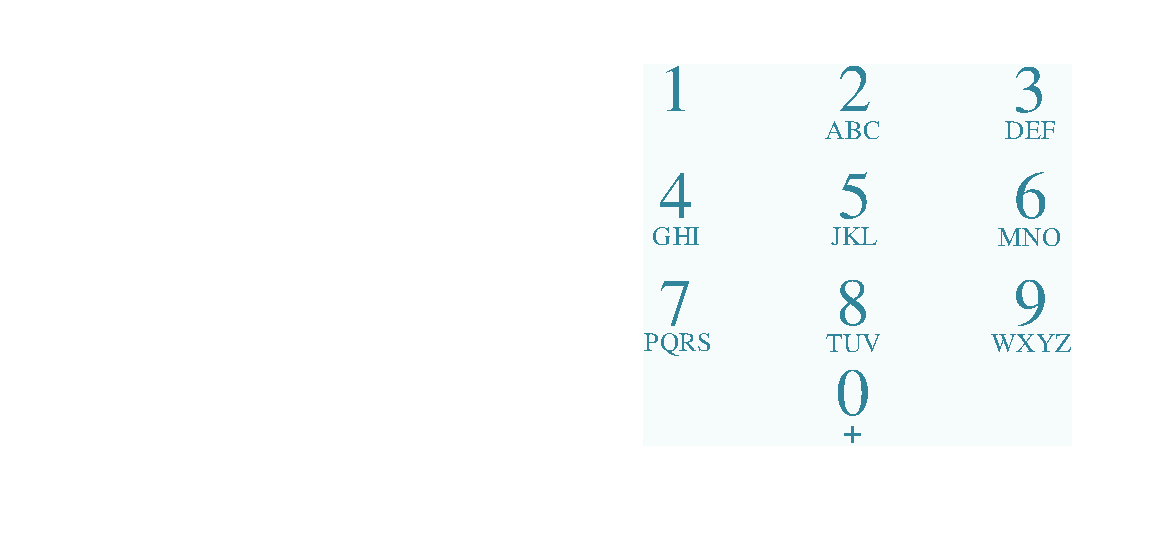
\includegraphics[width=\textwidth]{fig/pin_screen.pdf}\\
                \centering  (b) pin-based interface
                \end{minipage}
            }
            \caption{Pattern- (a) and pin-based (b) authentication interfaces.}
            \label{fig:unlock interface}
        \end{figure}

    \begin{figure}[!t]
        \centering
        \subfigure{
             \begin{minipage}[t]{0.22\textwidth}
                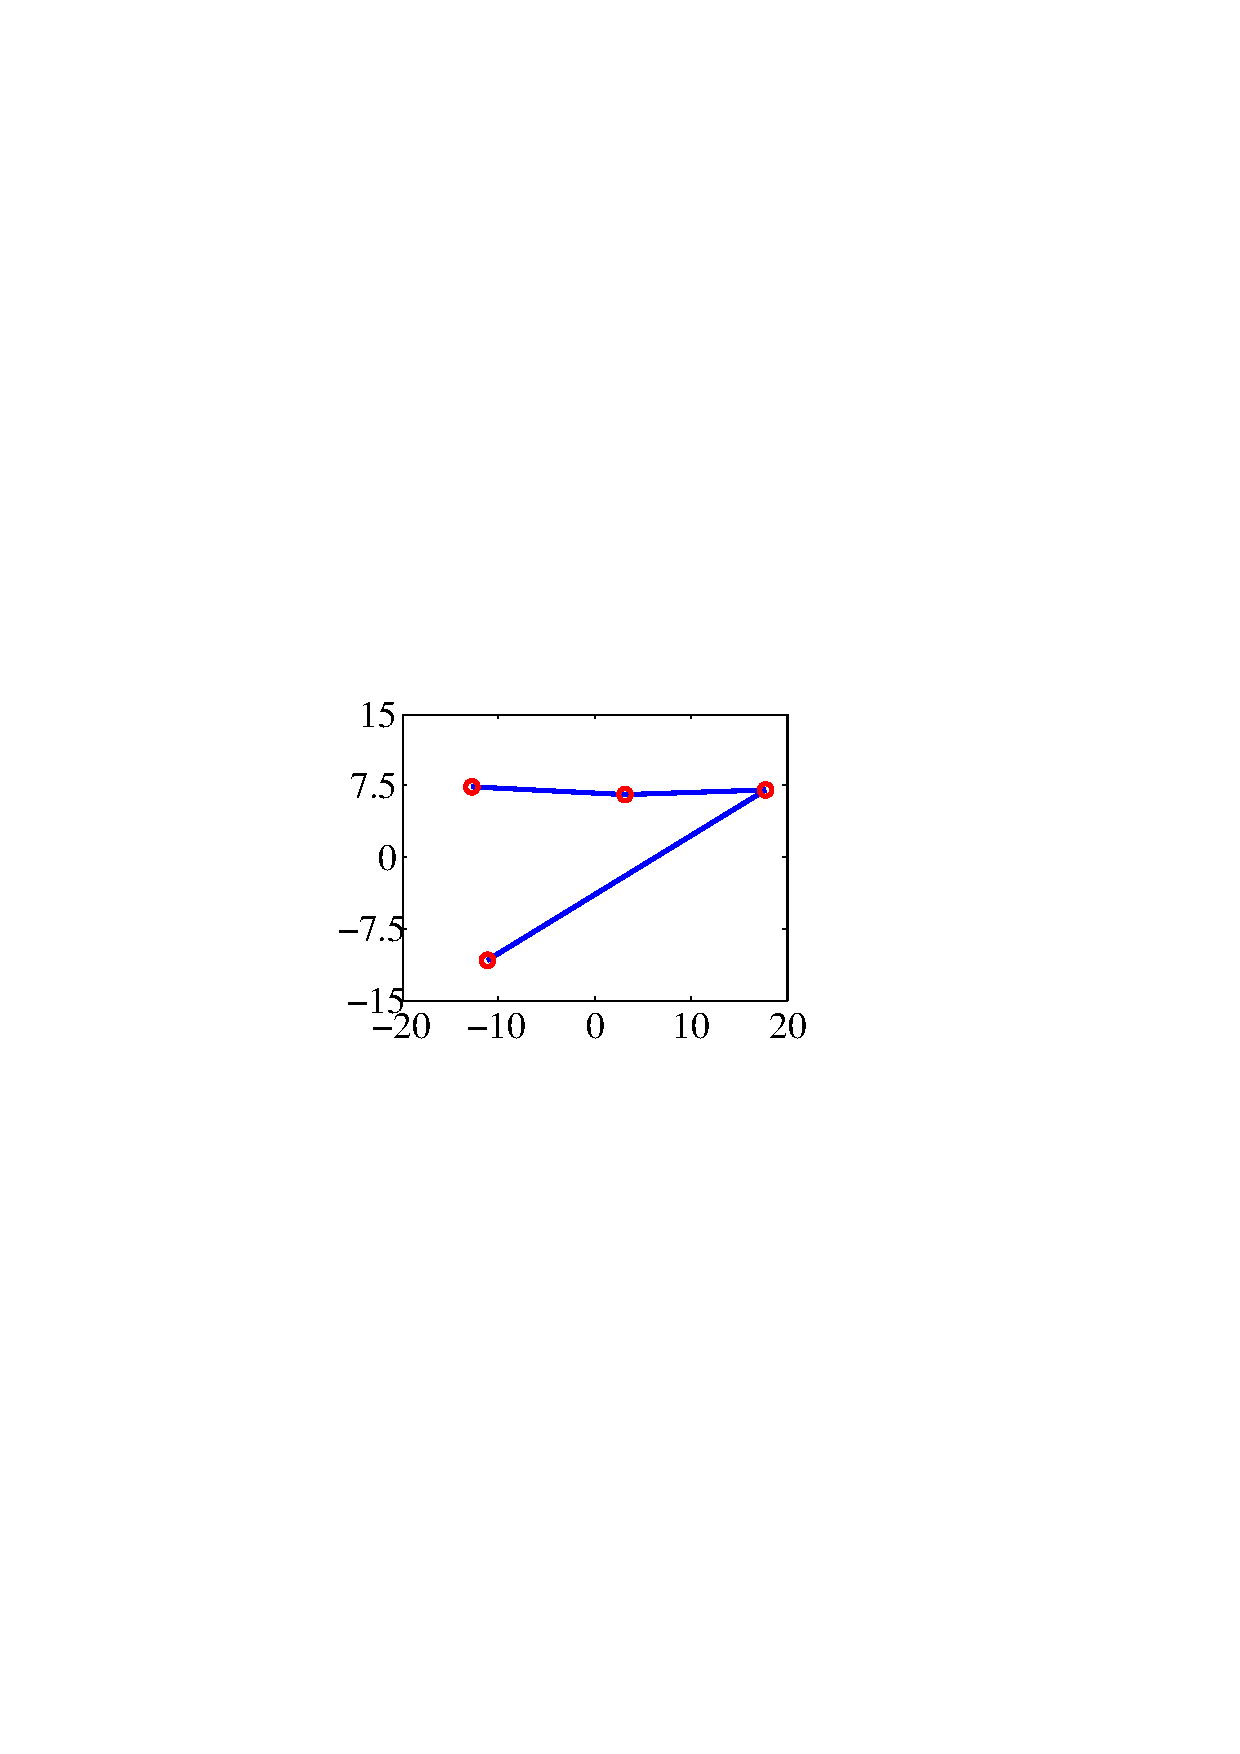
\includegraphics[width=\textwidth]{fig/pin_1234.pdf}\\
                \centering  (a) password: 1234
             \end{minipage}
        }
        \subfigure{
             \begin{minipage}[t]{0.22\textwidth}
                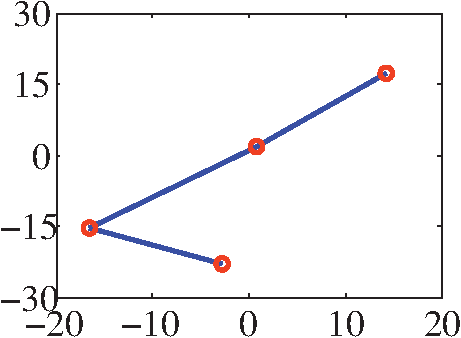
\includegraphics[width=\textwidth]{fig/pin_3570.pdf}\\
                \centering  (b) password: 3570
             \end{minipage}
        }
        \caption{Examples of tracked fingertip trajectory comprised of touching points. The red circle represents the touching points.}
        \label{fig:pins_trajectory}
    \end{figure}

    \subsection{Attacking PIN-base Passwords}
    \label{section: attacking-pin-passwords}
        \noindent \textbf{Result 9:} \emph{PIN-based passwords are also
        vulnerable under our video-side channel attack. We can break
        over 85\% of the pin-based passwords within five attempts using a
        variant method based on our approach.}

        An interesting question to ask is, could this method be used to attack PIN-based passwords? To answer this
        question, we apply our attacking method on 30 4-digital passwords. Among these passwords, 12 of them are most
        common used passwords (given by a PIN analysis survey conducted by Berry~\cite{Nick_pin_analysis}). The
        remaining passwords are randomly selected. For each password, we ask our participants to type in the password
        on a Xiaomi MI4 phone. Table~\ref{tab:PIN-based passwords} lists all PIN-based passwords considered in this
        experiment. Figure~\ref{fig:unlock interface} shows the subtle differences between the PIN-based keypad and the
        Android pattern grid. In this experiment, we used an IPhone4S phone to record the video from three angles of
        the target device: the
        left-front, front and right-front. The filming distance is 2 meters.

    \begin{figure}[!t]
        \centering
        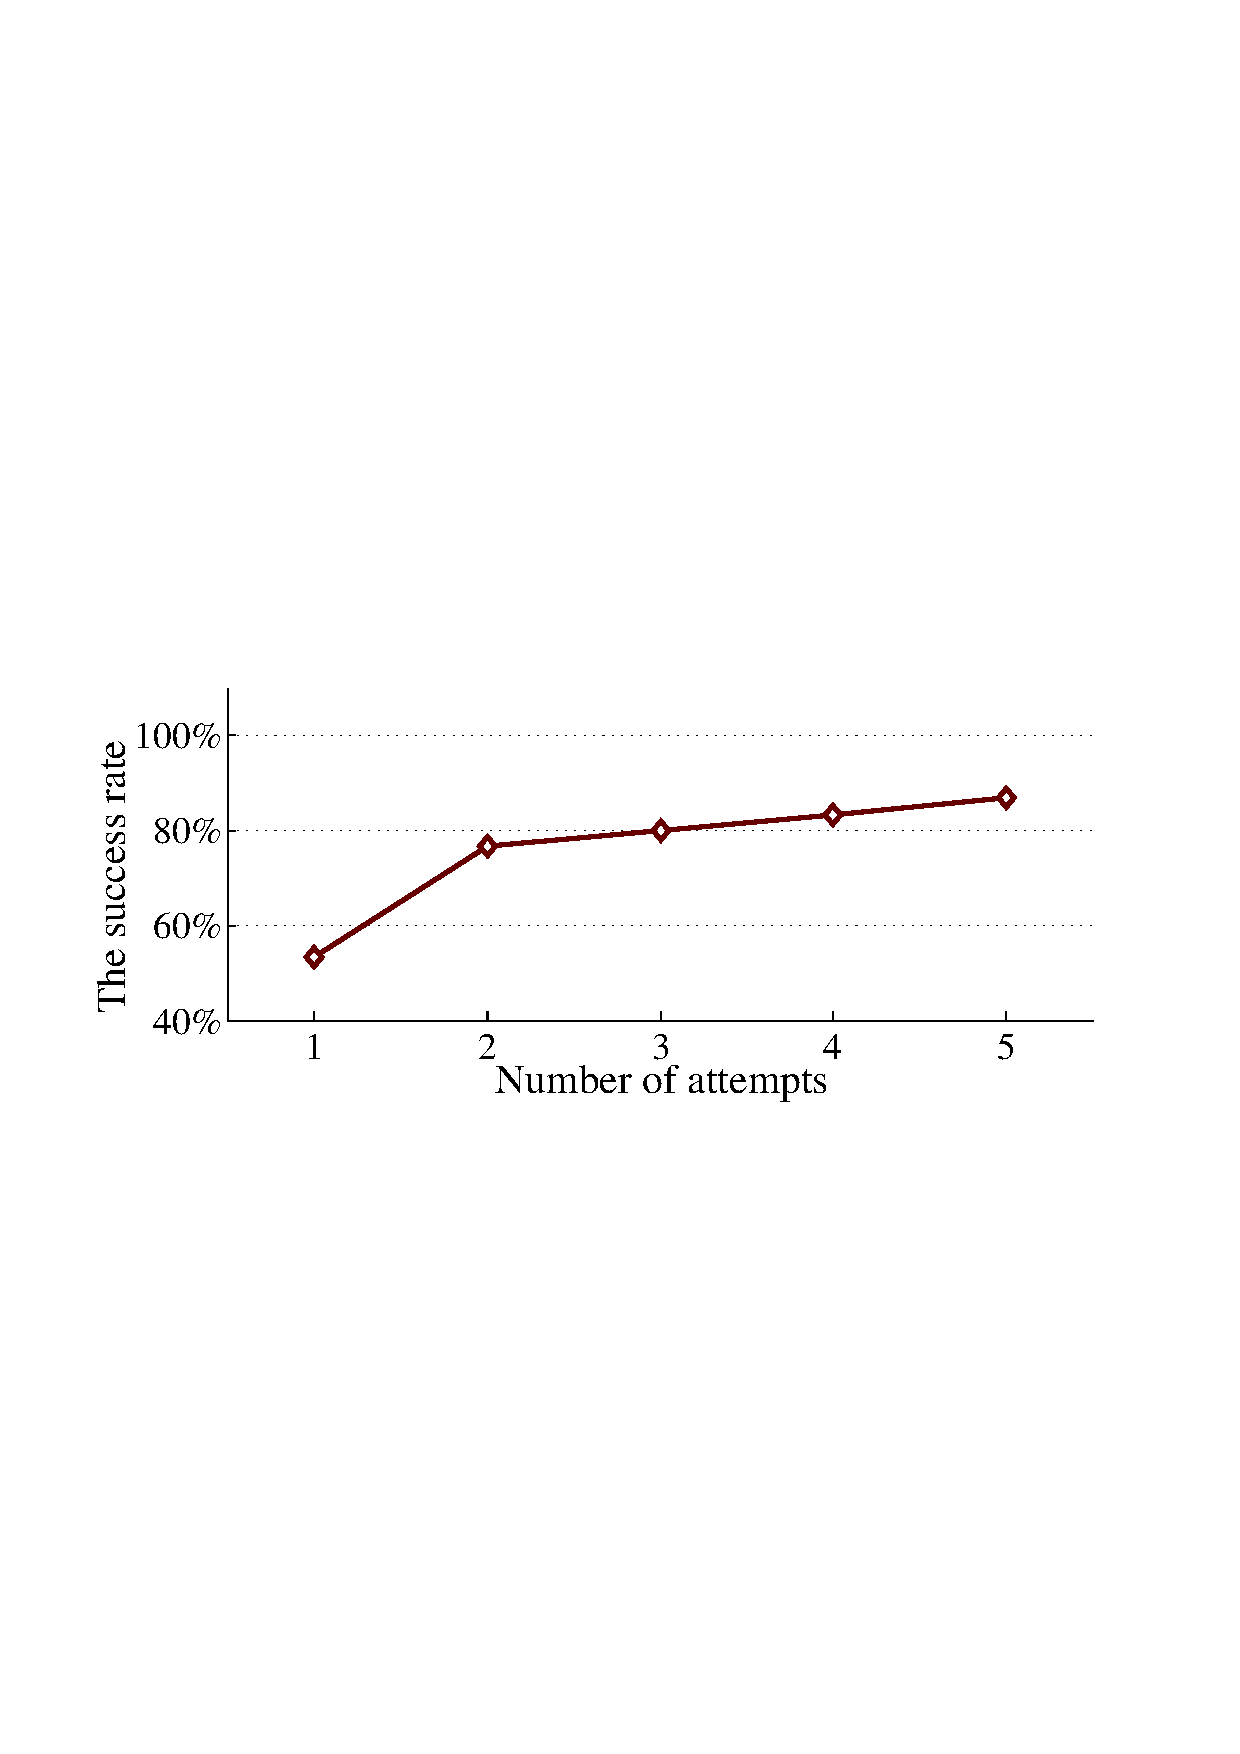
\includegraphics[width=0.5\textwidth]{fig/pin_results}\\
        \caption{The success rate of cracking PIN-based passwords with different number of attempts.}
        \label{fig:pin_results}
    \end{figure}

    \begin{figure}[!t]
        \centering
        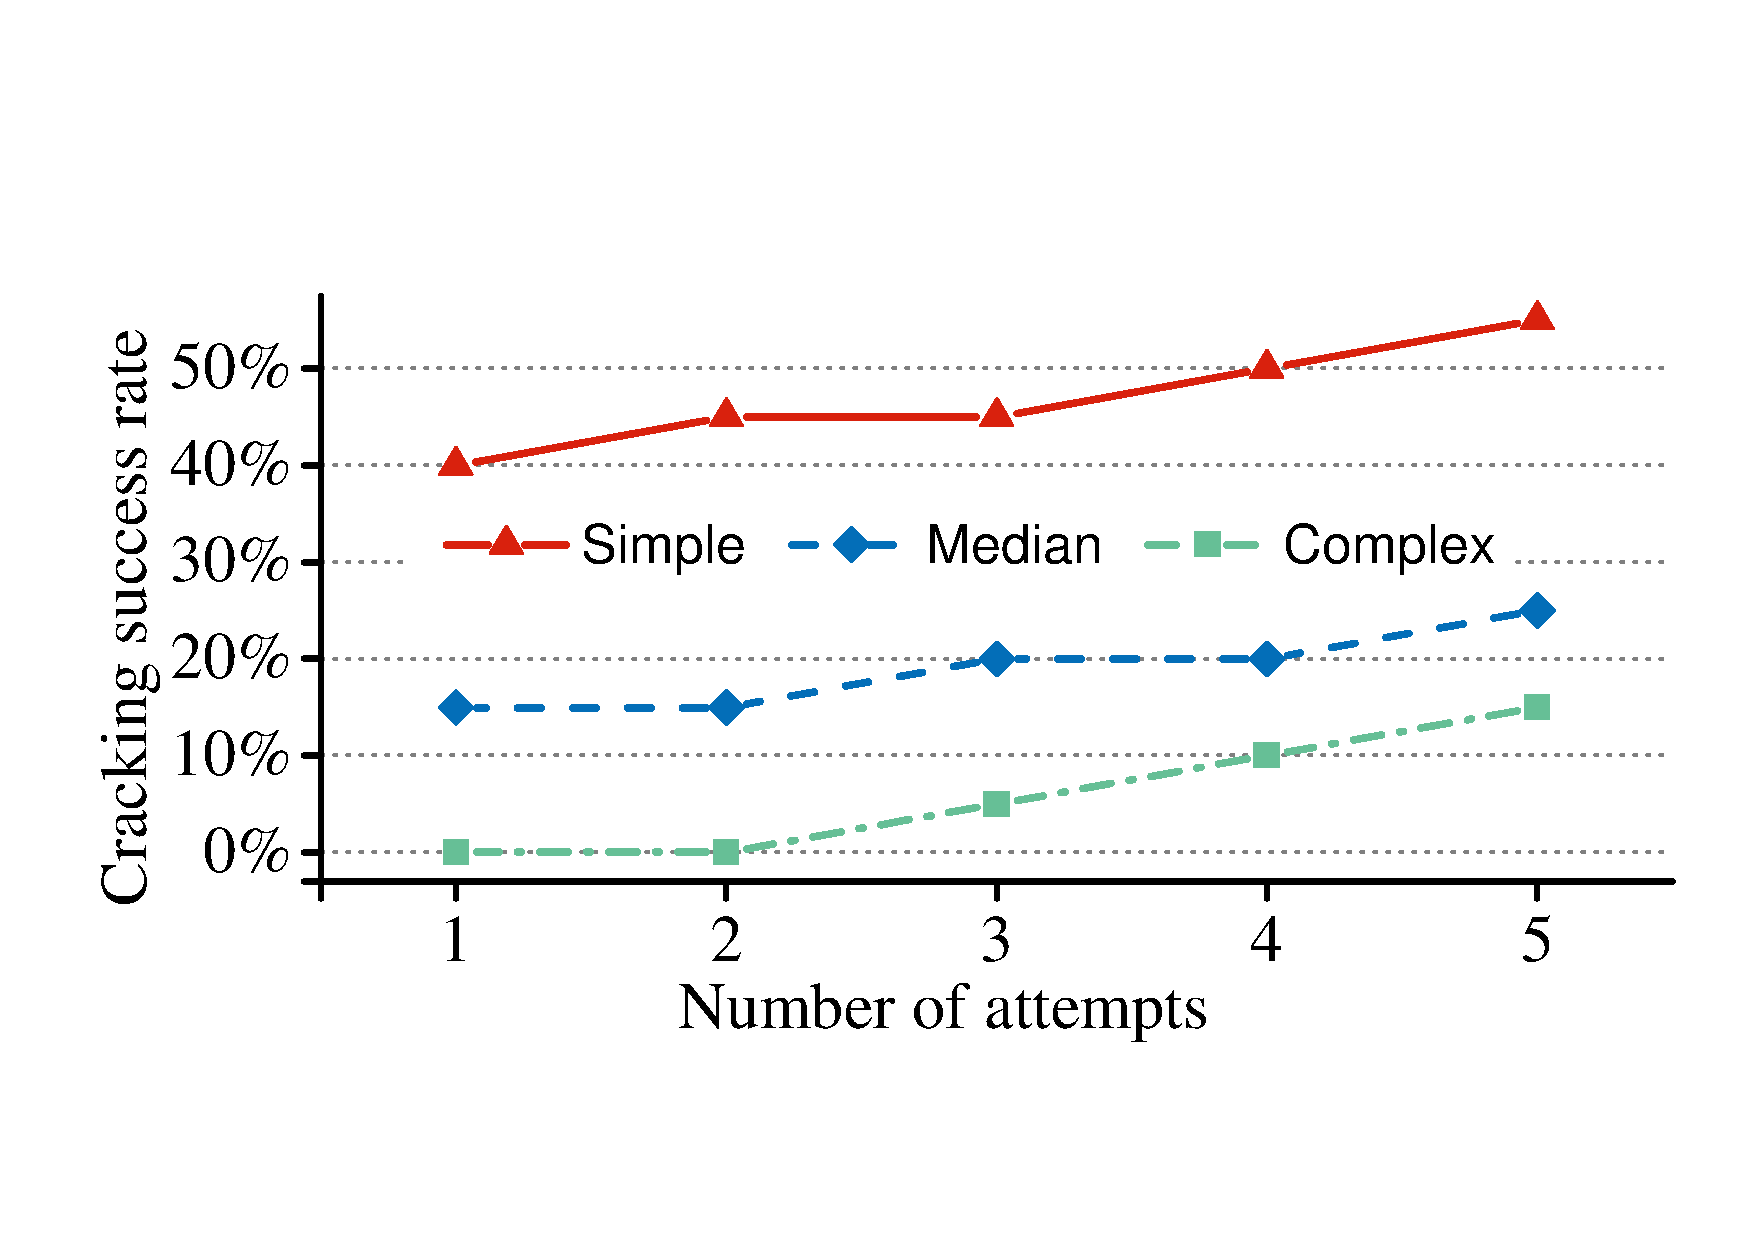
\includegraphics[width=0.5\textwidth]{fig/finger-only}\\
        \caption{The cracking success rate drops significantly when the video footage only captures the user's fingertip.}
        \label{fig:finger-only}
    \end{figure}

        \noindent \textbf{Variant Methodology.} Because the differences
        between the PIN-based password, we need to adapt our method. The two
        main differences are summarized as follow: (1) the number of the
        touch dots is different; and (2) each dot on the PIN pad can be
        visited multiple times, while each dot can only be visited once on
        pattern lock. The later difference requires us to identify dots that
        have been visited multiple times.  Our preliminary experiments
        suggest that we can reconstruct the trajectory of PIN-based password
        by connecting the touching points\footnote{Touching points are the
        points that are tracked when the user's fingertip touches the screen.}. We
        can obtain the location of touching point by tracking the up-and-down
        motion direction of the fingertip. This is inspired by the prior work
        conducted by Shukla~\emph{et al.}~\cite{shukla2014beware}. To reconstruct
        PIN-based passwords, our attacking method records some additional
        geometric information, including the direction and length
        information. Figure~\ref{fig:pins_trajectory} shows the tracked
        fingertip trajectory using the new attacking method.

        Figure~\ref{fig:pin_results} shows the
        results of applying our attacking method to PIN-based passwords.
        Using first attempt, the success rate is  53.3\% because most of
        evaluated passwords have two or more candidate patterns. However, the
        success rate increases with more attempts and reaches 86.7\% using 5
        attempts. After five attempts, our method fails to reconstruct four
        passwords. For two of failed passwords, our approach produces more
        than five candidate passwords; and for the other two, our approach
        incorrectly locates one of the touching points due to  blur
        motion of the video footage. Overall, our method can achieve a high
        cracking success rate for PIN-based passwords. Our findings are in
        line with prior works on video-based side channel for PIN-based
        passwords~\cite{shukla2014beware}.

       % two passwords is because they have more than five candidate patterns and for remaining two ones is that we detected the wrong location of one touching point due to the blue motion of the video footage. We believe that the expert attacker is able to improve the success rate using more attempts.
%

\subsection{Limited Study}
\label{section: limited-study}

Our attacking method requires the user's fingertip and part of the device to be seen in the video footage.  As
described in Section~\ref{secction:shake}, this is essential for calculating the coordinates of the fingertip and for
camera shake calibration. An interesting question to ask is can we relax this requirement, i.e., how will the attack
perform if the video footage only captures the user's fingertip. If our findings
suggest that the success of the attack requires seeing part of the device, a potential countermeasure is to educate users to cover their devices when entering their patterns.
As a limited study, in this experiment we ensure the video only capture user's fingertip. This study is performed on 20 patterns randomly selected by our participants.

Figure~\ref{fig:finger-only} shows the success rate of our attacking method is low when the device is not seen in the video footage.
This is large due to the fact the negative impact of the camera shake on tracking fingertip movement trajectory (see also Section~\ref{secction:shake}).
With only the fingertip location, the attacking method fails to cancel the camera shake effect, leading to low quality fingertip movement trajectory
which in turn translates to a poor success rate (less than 50\%, 30\% and 20\% for simple, medium and complex patterns respectively).


